\documentclass[aps,prl,reprint,superscriptaddress,longbibliography,nofootinbib,floatfix]{revtex4-2}
\usepackage{amsmath}
\usepackage{amssymb}
\usepackage{amsthm}
\usepackage{array}
\usepackage{xcolor}
\usepackage{tikz}
\usetikzlibrary{decorations.pathreplacing,decorations.pathmorphing}
\usepackage{graphicx}
\usepackage[colorlinks=true,linkcolor=blue,citecolor=blue,urlcolor=blue]{hyperref}

\newtheorem{theorem}{Theorem}
\newtheorem{lemma}{Lemma}
\newtheorem{corollary}{Corollary}
\newtheorem{conjecture}{Conjecture}
\theoremstyle{definition}
\newtheorem{definition}{Definition}

\newcommand{\ket}[1]{|#1\rangle}
\newcommand{\bra}[1]{\langle#1|}
\newcommand{\tr}{\operatorname{tr}}

\begin{document}

\title{A Parameter-Free Candidate for the Fine-Structure Constant from Entangled Qudits}

\author{A. D. Wissner-Gross}
\email{alexwg@alexwg.org}
\homepage{https://www.alexwg.org}
\noaffiliation
\date{October 23, 2026}

\begin{abstract}
We derive an exact candidate for the fine-structure constant $\alpha(0)$ from one parameter-free quantum-information axiom: nothing exists but finitely many maximally entangled pairs of finite-dimensional systems, some shared, known only by distilling them. Its one readable link with an acting central charge, a qutrit with a qubit, has the Standard Model gauge group $(SU(3)\times SU(2)\times U(1))/\mathbb{Z}_{6}$ and two-point function $(79+48\sqrt{2}+42\sqrt{3}+3\sqrt{6})/31104=1/137.035\,999\,190\ldots$. We conjecture that this link is the elementary link of the photon, making the number $\alpha(0)$, $0.6\sigma$ from CODATA 2022. Lean~4 checks the computation.
\end{abstract}

\maketitle

\emph{Introduction.}---The fine-structure constant at zero momentum transfer, $\alpha(0)$, is known to a tenth of a part per billion~\cite{fan2023,morel2020,parker2018,codata2022}, yet the Standard Model takes it from experiment. A derivation of $\alpha(0)$ would, almost by definition, draw on physics beyond the Standard Model, and the precision of the measurements, about ten significant figures for any candidate to match, could make $\alpha(0)$ an exquisite probe of that physics. Proposed closed forms for $\alpha(0)$ have a long history, and the serious ones foundered on what fixed their normalization, since the volume of a symmetric domain can be rescaled, and with it the number~\cite{wyler1969,wyler1971,robertson1971,gilmore1972}. A derivation of $\alpha(0)$ must therefore exhibit its one input and leave nothing to fix.

It must also compute the right quantity, and the on-shell scheme of quantum electrodynamics says which. For a massless spin-one field coupled to a conserved abelian charge, the coupling at zero transfer is universal~\cite{weinberg1964,weinberg1965}; the Ward identity $Z_{1}=Z_{2}$, equating the renormalizations of the vertex and of the charged field, reduces it to the vacuum polarization, $\alpha(0)=Z_{3}\,\alpha_{\mathrm{bare}}$, with $Z_{3}$ the renormalization of the gauge field and $\alpha_{\mathrm{bare}}$ the bare coupling~\cite{peskin1995}; and charged states of any mass decouple from this limit~\cite{appelquist1975}. One needs exactly one object with (i)~a conserved abelian charge obeying a Ward identity and (ii)~a two-point function with its pole at zero transfer, and then (iii)~its dressed-over-bare two-point function at that pole, the ratio of residues that is $Z_{3}$.

Three facts suggest where to look. First, a bounded region holds finitely many degrees of freedom~\cite{bekenstein1981,thooft1993,susskind1995}, and quantum theory and gravitation have both been reconstructed from information and entanglement~\cite{hardy2001,chiribella2011,jacobson1995,vanraamsdonk2010}. Second, the Standard Model gauge group $(SU(3)\times SU(2)\times U(1))/\mathbb{Z}_{6}$ is generated by local basis changes at the two ends of a qutrit maximally entangled with a qubit, namely $SU(3)$ at one end, $SU(2)$ at the other, and a relative phase that neither end owns. Third, bound entanglement, certifiable but undistillable, first becomes possible when the product of the two dimensions exceeds six~\cite{horodecki1996,phorodecki1997,horodecki1998,horodecki2009}, the bound beyond which positive maps between two systems need not decompose. Taken literally, in the spirit of Wheeler's ``it from bit''~\cite{wheeler1990}, they combine into a single axiom.

\emph{The model.}---This axiom is our model's only input:

\smallskip
\noindent\textbf{Axiom.} \textit{Nothing exists but finitely many maximally entangled pairs of qudits, some qudits shared, known only by distilling them.}
\smallskip

\noindent\textbf{Definitions.} A \emph{qudit} is a finite-dimensional quantum system, of dimension at least two, since a one-dimensional system cannot be entangled and so ends no pair. A \emph{pair}, or \emph{link}, of type $(d_{1},d_{2})$ joins qudits of dimensions $d_{1}$ and $d_{2}$ in the maximally entangled state on their common support, of dimension $m=\min(d_{1},d_{2})$,
\begin{equation}
\ket{\omega_{m}} = \frac{1}{\sqrt{m}}\sum_{i=1}^{m}\ket{i}\ket{i}.
\label{eq:pair}
\end{equation}
A qudit is \emph{shared} when it is an end of two or more pairs. Because a pure maximally entangled pair is uncorrelated with every third system, a shared qudit is carried as one copy per pair, each maximally entangled with its own partner, as in a projected entangled pair state~\cite{verstraete2004}, so monogamy is never violated. These are copies of a qudit, one per pair, not copies of a link, of which there is only ever one. The copies are still one qudit, the one the axiom shares, so exchanging two pairs at a shared qudit leaves it in place and moves only what sits at their far ends. To \emph{distill} two qudits is to project them onto $P_{m}=\ket{\omega_{m}}\!\bra{\omega_{m}}$, and its output is the pair of their type.

Here, \emph{distilling} generalizes entanglement distillation, which extracts maximally entangled pairs from many copies of a less entangled state by local operations and classical communication~\cite{bennett1996a,bennett1996b}. But every state is already maximally entangled, so there is nothing for copies or local operations to purify, and what remains is a single joint projection onto the pair state, on one copy and with no failure branch. It is the projection of entanglement swapping~\cite{zukowski1993}, which between pairs moves entanglement and adds none. In a laboratory, the same projection is a postselection, one outcome of a Bell measurement, obtained between two pairs of dimension $d$ with probability $1/d^{2}$. In our model, the complementary outcome is no configuration of the axiom, so the projection is the act itself. Postselection has been proposed as a law before, for the final state of black holes and for closed timelike curves~\cite{horowitz2004,lloyd2011}.

By the transpose identity $(A\otimes\openone)\ket{\omega_{m}}=(\openone\otimes A^{T})\ket{\omega_{m}}$, an operator at one end of a pair acts as its transpose at the other. The pair state therefore has the same form $\sum_{i}\ket{e_{i}}\ket{\bar{e}_{i}}/\sqrt{m}$ in every basis $\{\ket{e_{i}}\}$ of the support, with the complex-conjugate basis at the far end, so distilling picks out no basis. A \emph{matching}, a change of that basis by a unitary $U$ of the support, acts on the pair as $U\otimes\bar{U}$ and leaves it unchanged. Each pair has its own matching, so nothing lines up the bases of a shared qudit's copies. A \emph{read} is an act at one end of a pair, the end at which it is taken. It distills the two ends in a basis of that end and passes the basis along the pair, leaving the far end at each element $\ket{e}$ in $\bra{e}\omega_{m}\rangle$, the conjugate of the part of $\ket{e}$ on the support, with no freedom. The basis it passes reaches the far end whole, but these states span only the support, so a read is taken at the larger end of a pair, or at either end when the two are equal. At an end of prime dimension $d$, such as a qubit or a qutrit, there is one read for each of the $d+1$ mutually unbiased bases of the clock and shift operators~\cite{wootters1989}. The traceless parts of their projectors, $d-1$ per basis, are mutually orthogonal, so no read repeats another, and together span all \mbox{$(d+1)(d-1)=d^{2}-1$} traceless observables of that end, three at a qubit (the Pauli matrices) and eight at a qutrit (the Gell-Mann matrices).

To \emph{fix} is to determine with certainty from a single copy, not to estimate an expectation value over many. Certainty leaves nothing open, so a read fixes two ends only when every consistent relation between them, a positive map between their operator algebras, is of a kind distillations carry. What is \emph{known} of a qudit is what its reads fix jointly, under every matching of its pairs and every exchange of its reads or of its pairs. Two reads fix their product jointly, and exchanging them returns the product times the phase by which they fail to commute. An exchange done twice is no exchange, so that phase must be a sign, and two anticommuting reads thus fix one thing more than either alone, their product, with their order as its sign. These five definitions, of a qudit, sharing, distilling, a read, and the known, spell out the axiom's terms, and their properties follow from it (Supplemental Material~\cite{SM}, Sec.~S1).

\emph{Measurement.}---Three consequences of the axiom settle our model's measurement theory. A \emph{configuration} is a set of links, some of them read, and its \emph{readout} is the number its reads deliver. First, the pair state is unchanged, or envariant~\cite{zurek2003}, under every matching, so every readout is invariant under their average, the isotropic twirl. Second, the pairs are finitely many and distilling creates no qudit, so no link between the same two qudits exists twice. A read therefore acts once on the one copy of the link it reads, and what matters is what a \emph{single} read fixes, not asymptotic distillability. Third, the operators invariant under every matching are spanned by $\openone$ and $P_{m}$~\cite{horodecki1999}, so a read delivers its pair projector and nothing finer.

The readout is then a normalized trace over the \emph{readout algebra} $R$, the operators the reads can reach, which are the whole operator space of each read link and, since no read sees the scalar part of an unread link, the traceless part of each unread link. What the reads insert into a readout is an operator on $R$, an \emph{insertion}, as an $n$-point function in field theory inserts $n$ fields into a state. A configuration may carry any number of reads, and this Letter needs two, those of a two-point function. The on-shell scheme of the Introduction compares the \emph{dressed} two-point function $G_{\mathrm{dressed}}$, with every interaction, to the \emph{bare} one $G_{\mathrm{bare}}$, with none. Here the \emph{bare insertion} is the identity of $R$, which weighs every direction of $R$ once, and the \emph{dressed insertion} $M$ weighs only the directions the reads fix, each at the amplitude it carries through the pairs it runs over (Theorem~\ref{thm:value} below). The readout of $M$ is~\cite{SM}
\begin{equation}
\langle M\rangle = \tr_{R}M/\dim R,
\label{eq:readout}
\end{equation}
and that of the bare insertion is one, so $\langle M\rangle$ is itself the dressed-over-bare ratio $G_{\mathrm{dressed}}/G_{\mathrm{bare}}$.

\emph{Which links can be read.}---A read meets a pair ket, pure and maximally entangled, so its projection onto the pair succeeds with probability one on the single copy, and that certainty is the bare unit of the readout. No state of the model is bound entangled, since every link is a pure maximally entangled state, distillable in every dimension. What a read can fail to fix is therefore not a state but a relation between the two ends of a type. A consistent relation, a positive map between the operator algebras of two ends, carries every description of one end to a description of the other, and the matchings are its unitary cases. Reads carry operators across a link in two ways, directly by their projection and the matchings, which are completely positive, and to the far end by the transpose identity. Every map that reads compose is therefore \emph{decomposable}, a completely positive map plus a completely positive map after the transpose~\cite{SM}. Call a type \emph{readable} when every positive map between its ends is decomposable, so that reads carry every consistent relation between them, and \emph{dark} otherwise.

By the definition of fix, a single read fixes the ends of a pair exactly when its type is readable. Every positive map is decomposable at $(2,2)$~\cite{stormer1963} and $(2,3)$~\cite{woronowicz}. Non-decomposable maps exist at $(2,4)$~\cite{woronowicz} and $(3,3)$~\cite{choi1975}, and they embed in every type with $d_{1}d_{2}\geq 8$; no product of two integers $\geq 2$ equals seven. So a type of dimensions $d_{1},d_{2}\geq 2$ is readable if and only if $d_{1}d_{2}\leq 6$, the \emph{read cap}, and the readable types are $(2,2)$ and $(2,3)$, of which $(2,3)$ alone has unequal ends.

Through the Choi--Jamio{\l}kowski correspondence~\cite{choi1975cp,jamiolkowski1972}, the maps reads cannot carry are the witnesses of entanglement with positive partial transpose~\cite{horodecki1996,phorodecki1997}, which no standard distillation reaches~\cite{horodecki1998}, so a dark type has a sector that standard distillation never reaches, though each of its links stays maximally entangled. Standard distillation reaches every entangled state of a type exactly when $d_{1}d_{2}\leq 6$~\cite{horodecki1999,horodecki2009}, the bound at which a single read fixes the type.

A second route gives the same cap, if the far end of a read must hold the passed basis as its own~\cite{SM}. With reads taken at qubits and qutrits, a read spans no end of dimension four or more. A read also hands its basis to the far end complex-conjugated, by the transpose identity, and the far end can take that basis as its own only if a matching undoes the conjugation, as $\sigma_{y}$ does at a qubit and no unitary does at a qutrit. So the far end of a read is a qubit, which leaves exactly the readable types $(2,2)$ and $(2,3)$, with $(2,3)$ read at its qutrit end.

\emph{The charge.}---The identification algebra of a $(d_{1},d_{2})$ link is $su(d_{1})\oplus su(d_{2})\oplus u(1)$, the block-diagonal traceless anti-Hermitian operators on $\mathbb{C}^{d_{1}}\oplus\mathbb{C}^{d_{2}}$, the infinitesimal basis changes at its two ends, and an element $\xi=\xi_{1}\oplus\xi_{2}$ acts on the link as $\xi_{1}\otimes\openone+\openone\otimes\xi_{2}$. Its center is spanned by
\begin{equation}
\mathcal{Q} = i\,\mathrm{diag}\big(d_{2}\openone_{d_{1}};\,-d_{1}\openone_{d_{2}}\big),
\label{eq:Q}
\end{equation}
which acts on the whole link, the pair ket $\ket{\omega_{m}}$ included, as the scalar $i(d_{2}-d_{1})$. At $(2,2)$ it vanishes; at $(2,3)$ it is $i$. So exactly one readable type carries an acting central charge, and its algebra is $su(3)\oplus su(2)\oplus u(1)$. This is the Lie algebra of $S(U(3)\times U(2))$, the block-diagonal unitaries of determinant one on $\mathbb{C}^{2}\oplus\mathbb{C}^{3}$, to which its operators exponentiate. The group $S(U(3)\times U(2))\cong(SU(3)\times SU(2)\times U(1))/\mathbb{Z}_{6}$ is the Standard Model gauge group in the global form realized in $SU(5)$~\cite{baez2010}, and $\mathcal{Q}=6iY$ is its hypercharge generator, $Y=\mathrm{diag}(\tfrac{1}{2},\tfrac{1}{2};\,-\tfrac{1}{3},-\tfrac{1}{3},-\tfrac{1}{3})$. Inside it, the stabilizer of the pair has dimension four, with center the unbroken generator $\mathcal{U}=i\,\mathrm{diag}(1,1;\,-1,-1,0)$~\cite{SM}.

The charge is conserved. Up to scale, the only functional of the open ends of a configuration that every matching preserves and that sees no global phase is the count of $\mathcal{Q}$, and every read or join changes the open ends by a matched ket--bra pair, so the count is unchanged. The count sums to zero over all directions of the two ends, which is the tracelessness of $\mathcal{Q}$, while the link matches one direction of each end, which is why $\mathcal{Q}$ acts on the pair ket as $i$. Because the twirl fixes $\mathcal{Q}$, its dressed and bare insertions agree, $Z_{1}=Z_{2}$~\cite{SM}.

\emph{The object.}---The charge meets requirement~(i) of the Introduction, a conserved abelian charge with $Z_{1}=Z_{2}$, so the coupling reduces to $Z_{3}$, the dressed-over-bare two-point function of requirement~(iii). That ratio is the readout $\langle M\rangle$ of Eq.~(\ref{eq:readout}), and it is the number the conjecture below identifies with $\alpha(0)$. What remains is to say which configuration is the link's two-point function and to count its readout. A two-point function has two insertions on one state. In our model, the two insertions are two reads of the link, and the state is the link itself, present as a third link of the same type at the same shared qudit and left unread, since reading it would be a third insertion (Fig.~\ref{fig:link}). This is the model's definition of a two-point function~\cite{SM}. By the definition of a read, the reads are taken at the qutrit end, the \emph{end rule}. A qutrit-end read fixes the qubit's state at every basis element, whereas a qubit-end read would reach the qutrit only on the two-dimensional support, missing its third direction, the direction the unbroken generator $\mathcal{U}$ leaves at zero.

\begin{theorem}[Uniqueness]
\label{thm:object}
Among the configurations at a shared qudit whose read links are readable, exactly one is a two-point function, is read at the qutrit end, and carries an acting central charge on every link: a shared qutrit with three links to qubits, two of them read. We call it the \emph{object}.
\end{theorem}

\begin{proof}[Proof sketch]
The acting charge leaves only $(2,3)$ links, the end rule puts the qutrit at the shared end, and the two-point function takes two read links and one unread link of that type. The full proof, in Sec.~\ref{sec:s-config} of the Supplemental Material, enumerates these configurations, and the Lean file checks it~\cite{SM}.
\end{proof}

\emph{The count.}---Counting the object's readout, Eq.~(\ref{eq:readout}), takes three steps, the readout dimension $N$, the records, and the weight each record earns by surviving two exchanges. The shared qutrit is carried as one copy per link, at the two read links and the unread third, whose traceless part, the connected part of the pair projector, is the state. The readout dimension $N=\dim R$ follows from the two end dimensions alone, $(3^{2}-1)(2^{2}-1)=24$ at the unread link and $(3\cdot 2)^{2}=36$ at each read,
\begin{equation}
N = 24\cdot 36\cdot 36 = 31104.
\label{eq:N}
\end{equation}

\begin{figure}[t]
\centering
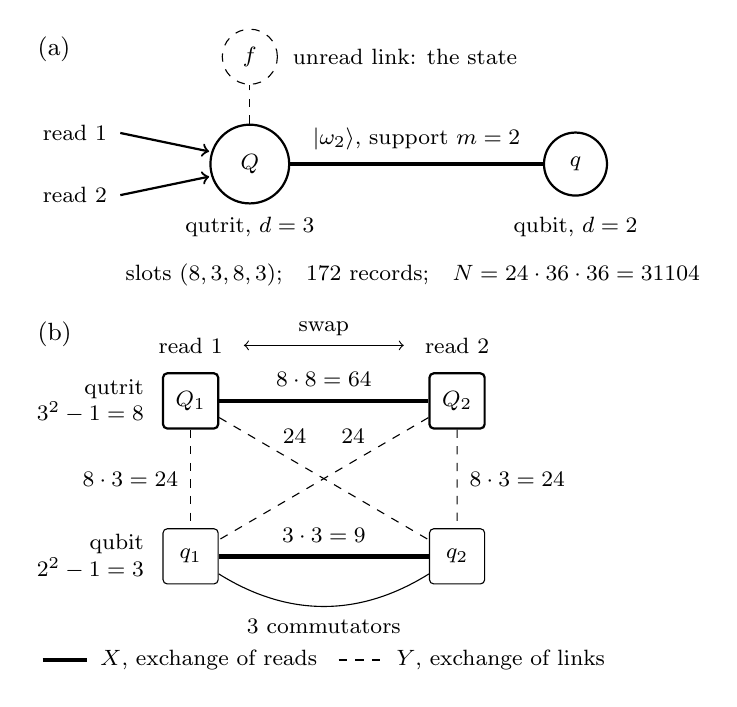
\begin{tikzpicture}[scale=0.94, every node/.style={font=\footnotesize}]
\node[draw, circle, minimum size=10mm, thick] (Q) at (0,0) {$Q$};
\node[draw, circle, minimum size=8mm, thick] (q) at (4.4,0) {$q$};
\node[draw, dashed, circle, minimum size=7mm] (f) at (0,1.45) {$f$};
\draw[very thick] (Q) -- node[above=1pt] {$|\omega_{2}\rangle$, support $m=2$} (q);
\draw[dashed] (Q) -- (f);
\node[anchor=west] at (0.45,1.45) {unread link: the state};
\node at (0,-0.85) {qutrit, $d=3$};
\node at (4.4,-0.85) {qubit, $d=2$};
\draw[->, thick] (-1.75,0.42) -- (-0.55,0.17);
\draw[->, thick] (-1.75,-0.42) -- (-0.55,-0.17);
\node[anchor=east] at (-1.8,0.42) {read 1};
\node[anchor=east] at (-1.8,-0.42) {read 2};
\node[align=center] at (2.2,-1.5) {slots $(8,3,8,3)$;\quad $172$ records;\quad $N = 24\cdot 36\cdot 36 = 31104$};
\node[anchor=north west, font=\small] at (-3.0,1.85) {(a)};
\begin{scope}[shift={(-0.8,-5.3)}, slot/.style={draw, rectangle, rounded corners=1.5pt, minimum size=7mm, inner sep=1pt}]
\node[slot, thick] (Q1) at (0,2.1) {$Q_{1}$};
\node[slot, thick] (Q2) at (3.6,2.1) {$Q_{2}$};
\node[slot] (q1) at (0,0) {$q_{1}$};
\node[slot] (q2) at (3.6,0) {$q_{2}$};
\draw[line width=1.6pt] (Q1) -- node[above=1pt] {$8\cdot 8=64$} (Q2);
\draw[line width=1.6pt] (q1) -- node[above=1pt] {$3\cdot 3=9$} (q2);
\draw[dashed] (Q1) -- node[left=1pt] {$8\cdot 3=24$} (q1);
\draw[dashed] (Q2) -- node[right=1pt] {$8\cdot 3=24$} (q2);
\draw[dashed] (Q1) -- node[pos=0.27, above right=-1pt] {$24$} (q2);
\draw[dashed] (Q2) -- node[pos=0.27, above left=-1pt] {$24$} (q1);
\draw (q1) to[bend right=32] node[below=1pt] {$3$ commutators} (q2);
\node at (0,2.85) {read 1};
\node at (3.6,2.85) {read 2};
\draw[<->] (0.72,2.85) -- node[above=0pt] {swap} (2.88,2.85);
\node[align=right, anchor=east] at (-0.5,2.1) {qutrit\\$3^{2}-1=8$};
\node[align=right, anchor=east] at (-0.5,0) {qubit\\$2^{2}-1=3$};
\draw[line width=1.6pt] (-2.0,-1.4) -- (-1.4,-1.4);
\node[anchor=west] at (-1.35,-1.4) {$X$, exchange of reads};
\draw[dashed] (2.0,-1.4) -- (2.6,-1.4);
\node[anchor=west] at (2.65,-1.4) {$Y$, exchange of links};
\end{scope}
\node[anchor=north west, font=\small] at (-3.0,-2.0) {(b)};
\end{tikzpicture}
\caption{(a)~The object: a qutrit--qubit link in the maximally entangled state $|\omega_{2}\rangle$ on its two-dimensional common support, read twice at the shared qutrit $Q$ (once on each of two links of this type, drawn as one), with a third, unread link of the same type, to the qubit $f$, carrying the state. Each read places a letter, a basis element of the traceless observables of an end, at either end of its link, its two slots, with $3^{2}-1=8$ letters at the qutrit and $2^{2}-1=3$ at the qubit, giving the slots $(8,3,8,3)$ and $172$ measurement records. The readout dimension is the traceless part of the unread link ($24 = 8\cdot 3$) times the operator space of the link at each read ($36 = 9\cdot 4$). (b)~The four slots as the corners of a square, with $Q_{1}$, $Q_{2}$ the shared qutrit's copies at the two read links and $q_{1}$, $q_{2}$ the two read qubits, each with the letters of its end. An edge is a pair of slots, not a link, and carries one product record for each letter at one end and each at the other, $64+9+4\cdot 24=169$ in all. The arc adds the $3$ commutator records, one for each pair of qubit letters, for $172$ in all. It joins the qubits only, since two reads in different bases anticommute at a qubit and no two reads anticommute at the qutrit, whose dimension is odd. Swapping the reads maps the solid edges to themselves, where $X$ acts, and the dashed edges to each other in pairs, where $Y$ acts [Eq.~(\ref{eq:s-exchanges})]; the records of the arc survive both. Tables~\ref{tab:sectors} and~\ref{tab:s-slotpairs} sort the records.}
\label{fig:link}
\end{figure}


\emph{The records.}---Each insertion is placed by a read on its link, at its own end directly or at the far end by the transpose identity, and what it places at an end is a traceless observable there, in the span of the traceless parts of the read projectors. We call an element of the basis of these observables a \emph{letter}, and each end of a read link, a place where a read puts a letter, a \emph{slot}. A qutrit end has $3^{2}-1=8$ letters, the Gell-Mann matrices, and a qubit end has $2^{2}-1=3$, the Pauli matrices, so the two read links give four slots, the qutrit copy $Q_{1}$ and qubit $q_{1}$ of the first and $Q_{2}$ and $q_{2}$ of the second, with $(8,3,8,3)$ letters. A \emph{measurement record} carries the two insertions as two letters. Two letters at the same slot act on the same end, where their product is a multiple of the identity plus one traceless observable, a single insertion. So the two letters of a record sit at different slots [Fig.~\ref{fig:link}(b)], except in the commutator records below. The six pairs of slots give $24+24+64+24+24+9=169$ such operators, $48$ of them with both letters at the two ends of one read. Exchanging the two reads fixes $11$ of them and pairs the other $158$ into $79$ odd and $79$ even combinations. At a qubit two reads in different bases anticommute (the Weyl phase there is $-1$), so by the definition of the known their commutator is a further record, with their order as its sign. At the qutrit no two reads anticommute, since $AB=-BA$ would give $\det(AB)=-\det(BA)$ in odd dimension, and no such record arises. The exchange carries the commutator at one read's qubit to the same commutator at the other's, and of the two combinations only their difference reads the order sign $-1$ under it, so there are three \emph{commutator records}, $172$ records in all~\cite{SM}. The records span the joint record space of the two reads. The readout is invariant under the exchange, hence diagonal in its eigenbasis, so the exchange sorts that space into its two eigenspaces, keeping both, and does not quotient it~\cite{SM}.

\emph{Survival.}---Two commuting exchanges sort the records~\cite{SM}. The \emph{exchange of reads} $X$ acts on a record that carries two letters of one type, by exchanging those two reads. These are the $73$ products with both slots at one end and the three commutator records, whose two qubit letters it reorders. The \emph{exchange of links} $Y$ exchanges the two read links. As a map on qudits it leaves the shared qutrit in place, by the definition of sharing, and swaps the two read qubits, so it acts on the records it carries to other qudits, the $96$ products with one slot at each end and the three commutator records.

By the definition of the known, a record survives an exchange, reading $-1$, when the exchange returns it times its own sign, which is $+1$ for a product, whose two letters sit at distinct slots and commute, and the order sign $-1$ for a commutator record. Otherwise it reads $+1$. We number the records $r=1,\dots,172$ and write $X_{r},Y_{r}=\pm 1$ for what record $r$ reads under the two exchanges. A product thus survives when it is symmetric, and each commutator record survives both. A record that survives an exchange is therefore the same, up to its own sign, whichever of the two reads or two links holds it. This echoes quantum Darwinism, in which a record is objective when many fragments of an environment hold it alike~\cite{ollivier2004,zurek2009}, although here nothing decoheres and every link is a pure maximally entangled pair. The joint eigenspaces have the sizes in Table~\ref{tab:sectors}, and Fig.~\ref{fig:records} draws every record; the Supplemental Material also counts them by pair of slots and from the traces of the two exchanges~\cite{SM}.

The weights are those of the dressed insertion $M$ of Eq.~(\ref{eq:readout}), which weighs each record at the amplitude it carries through the pairs it runs over. A record that survives an exchange is fixed under it, up to its own sign, so at the end where the exchange acts the matchings carry its letter over all $d$ matched directions of the pair there (at the shared qutrit, the three directions of the pair $\ket{\omega_{3}}$ that joins its copies). Each direction has amplitude $1/\sqrt{d}$ in Eq.~(\ref{eq:pair}), so the record carries $d\cdot(1/\sqrt{d})=\sqrt{d}$ there, and its squared weight gains the factor $d$. At an end where it survives no exchange, the pair contributes one. A read is an act at the end at which it is taken, so the exchange of reads acts there, at the qutrit by the end rule, wherever the letters sit, and $X$ contributes $3$, at the qubit--qubit records too. The exchange of links moves only what sits at the far ends, the read qubits, and $Y$ contributes $2$. The two exchanges commute and act at distinct ends, so a record that survives both has squared weight $3\cdot 2=6$. In all, record $r$ has the squared weight
\begin{equation}
k_{r} = 3^{[X_{r}=-1]}\,2^{[Y_{r}=-1]} = \tfrac{1}{2}(2-X_{r})(3-Y_{r}).
\label{eq:gain}
\end{equation}
where $[\cdot]$ is one when the condition inside it holds and zero otherwise. A record enters the readout with weight $\sqrt{k_{r}}$, not $k_{r}$. A record carries the two insertions of the two-point function as two letters, and its weight is its matrix element over the matched directions; the Born square $k_{r}$ is the record composed with its adjoint, four letters, a four-point quantity rather than the two-point function~\cite{SM}.

\begin{figure*}[t]
\centering
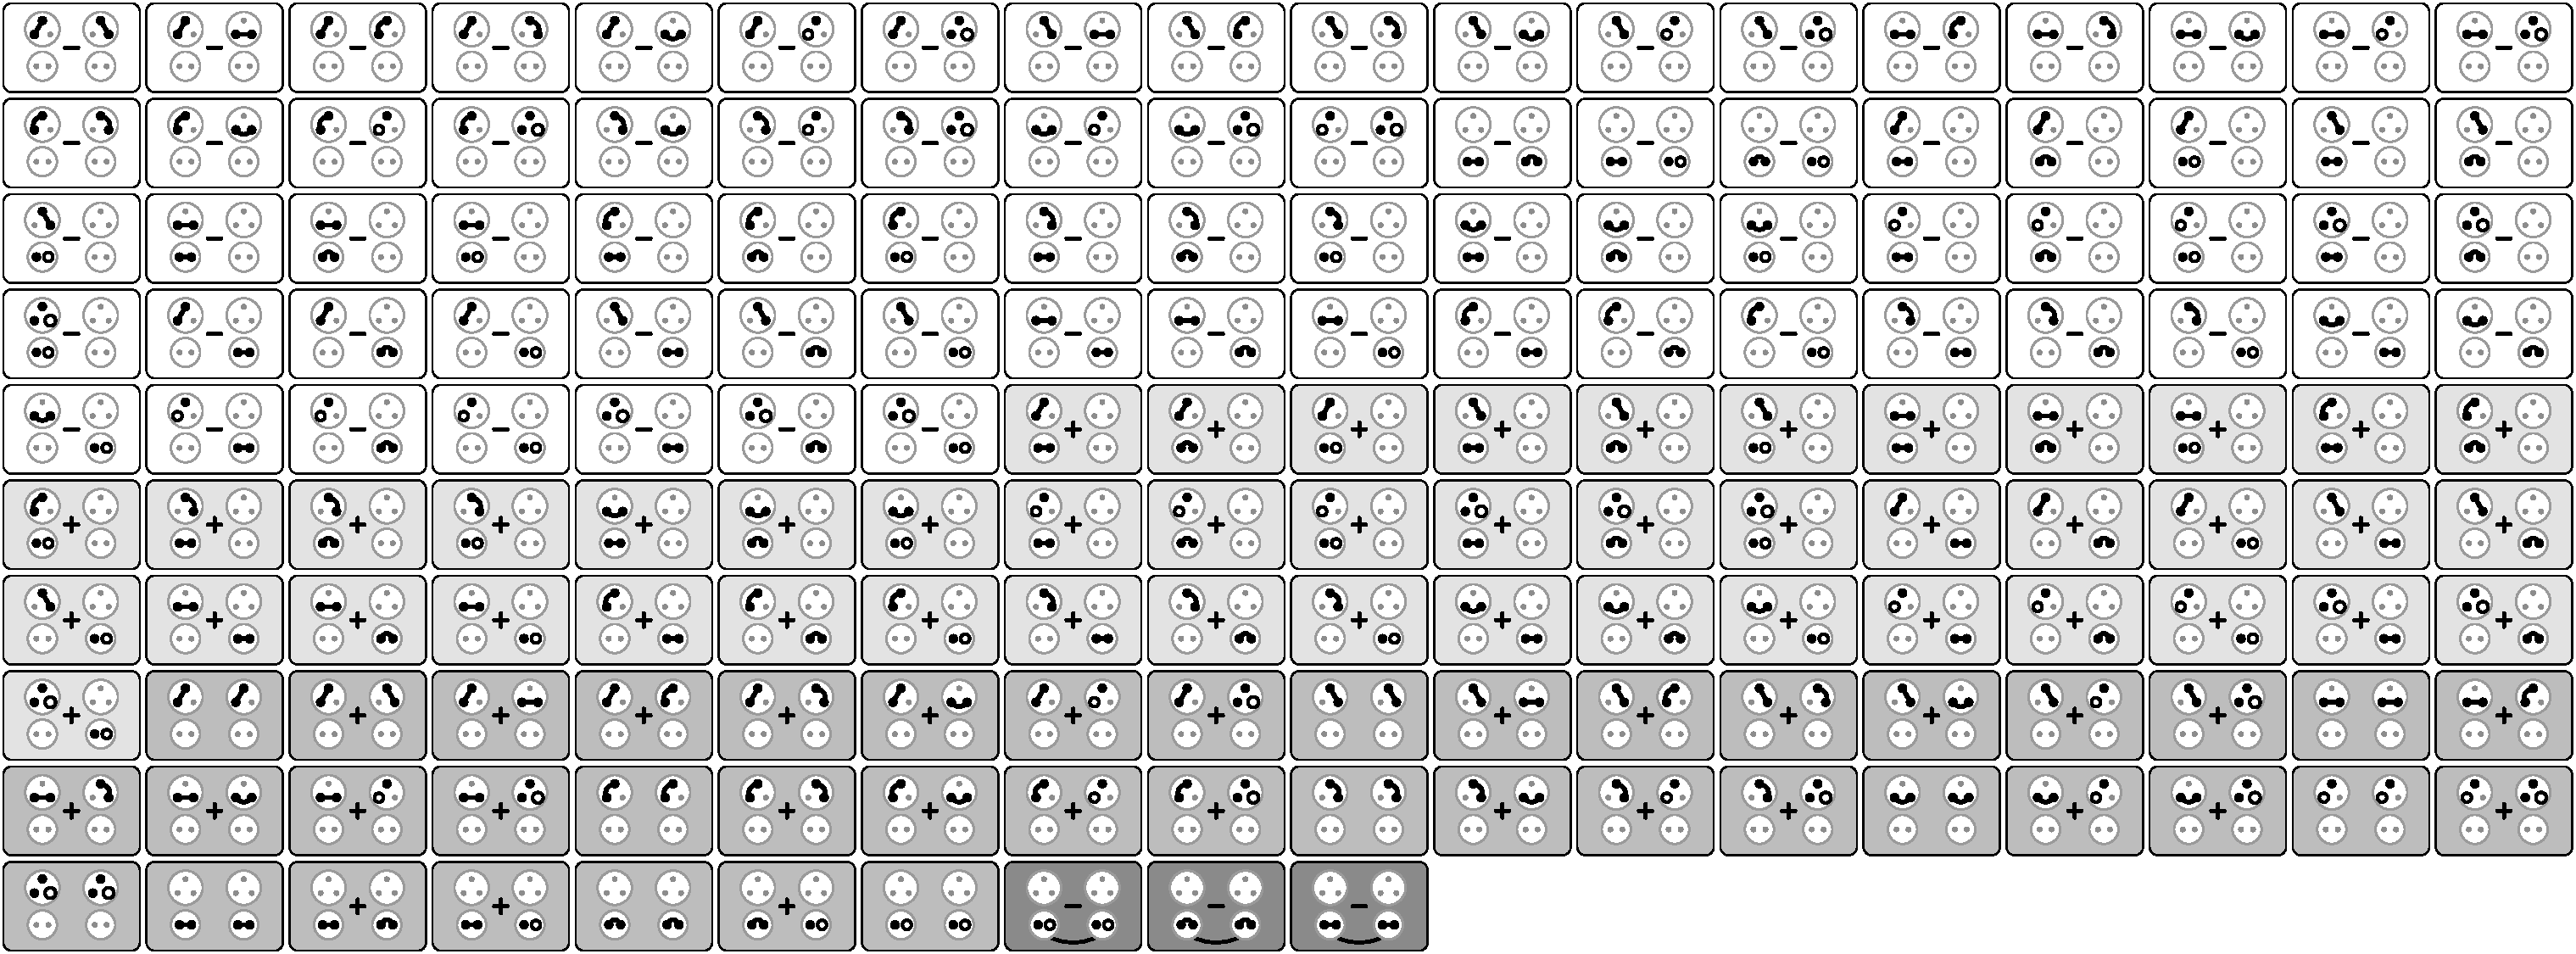
\includegraphics[width=\textwidth]{figures/records_atlas.pdf}
\caption{The $172$ measurement records of the object, one drawing each, on the square of slots of Fig.~\ref{fig:link}(b), with the qutrit copies $Q_{1}$, $Q_{2}$ above, with three dots, the basis directions, and the read qubits $q_{1}$, $q_{2}$ below, with two. Each record's two letters are drawn in their slots. A straight line joining two dots is a symmetric off-diagonal letter, a curved line an antisymmetric one, and filled and hollow dots a diagonal one. A $+$ or $-$ marks a record that is the drawing plus or minus its image under the exchange of the reads; a drawing with no sign is its own image. The three cells with an arc under the qubits are the commutator records, in which each qubit shows the commutator of two qubit letters, itself a single letter, and the record is the commutator at $q_{1}$ minus the same at $q_{2}$. Each cell's shade gives its weight $\sqrt{k_{r}}$ of Eq.~(\ref{eq:gain}), white for the $79$ records at $1$, light and then mid gray for the $48$ at $\sqrt{2}$ and the $42$ at $\sqrt{3}$, and dark gray for the $3$ at $\sqrt{6}$, the sectors of Table~\ref{tab:sectors}; the cells are sorted by weight. The drawings depend on the choice of basis; the counts and weights do not. The figure is drawn from the construction of the ancillary record script~\cite{SM}.}
\label{fig:records}
\end{figure*}


\begin{theorem}[Value]
\label{thm:value}
The dressed-over-bare two-point function of the object of Theorem~\ref{thm:object}, per unit of its conserved count, is
\begin{equation}
\frac{G_{\mathrm{dressed}}}{G_{\mathrm{bare}}} = \frac{1}{N}\sum_{r=1}^{172}\sqrt{k_{r}} = \frac{79+48\sqrt{2}+42\sqrt{3}+3\sqrt{6}}{31104}.
\label{eq:alpha}
\end{equation}
\end{theorem}

\begin{table}[b]
\caption{The $172$ records by the eigenvalues of the two exchanges. The weight $\sqrt{k_{r}}$ follows from Eq.~(\ref{eq:gain}); the sum of the weights is the numerator of Eq.~(\ref{eq:alpha}).}
\label{tab:sectors}
\begin{ruledtabular}
\begin{tabular}{lcccc}
records & $(X,Y)$ & number & $k_{r}$ & weight \\ \hline
odd & $(+,+)$ & $79$ & $1$ & $1$ \\
even, one slot at each end & $(+,-)$ & $48$ & $2$ & $\sqrt{2}$ \\
even, both slots at one end & $(-,+)$ & $42$ & $3$ & $\sqrt{3}$ \\
commutators & $(-,-)$ & $3$ & $6$ & $\sqrt{6}$ \\
\end{tabular}
\end{ruledtabular}
\end{table}

\begin{proof}[Proof sketch]
By Eq.~(\ref{eq:readout}) the readout is $\tr_{R}M/N$. Each record fixes one direction of $R$, its record operator at the two reads times the connected part of the unread link, and the $172$ directions are orthogonal. $M$ carries the weight $\sqrt{k_{r}}$ on the direction of each record and vanishes on the rest of $R$, which no read fixes, so each record contributes its weight. The bare function is $1$, the readout of the identity of $R$, and $Z_{2}/Z_{1}=1$. The full proof is in Sec.~\ref{sec:s-count} of the Supplemental Material, and the Lean file checks the value as its main theorem~\cite{SM}.
\end{proof}

We write $\alpha_{\mathrm{cand}}$ for this value, the candidate of the title, an element of $\mathbb{Q}(\sqrt{2},\sqrt{3})$ with rational coordinates $(79/31104,\,1/648,\,7/5184,\,1/10368)$ on the basis $(1,\sqrt{2},\sqrt{3},\sqrt{6})$. Its inverse is $\alpha_{\mathrm{cand}}^{-1}=137.035\,999\,189\,566\,155\ldots$, and Eq.~(\ref{eq:prediction}) below gives more digits. Equation~(\ref{eq:alpha}) is a sum of amplitudes over the records, the ways the two reads can carry the two insertions through the pairs, so it is the model's counterpart of the sum over Feynman diagrams, or over histories~\cite{feynman1948}, that dresses a two-point function~\cite{peskin1995}. It is finite and exact, with no expansion in a coupling and no integral to regulate.

\emph{Why this is the on-shell coupling.}---The correspondence with the on-shell scheme is set out row by row in the Supplemental Material~\cite{SM}. Read off the model, the two-point function factorizes as in field theory, $G_{\mathrm{dressed}}/G_{\mathrm{bare}}=Z_{3}(Z_{2}/Z_{1})^{2}\alpha_{\mathrm{bare}}$. The bare coupling is $\alpha_{\mathrm{bare}}=1$, the certainty with which a read's projection onto a pair ket succeeds, the bare unit of the readout~\cite{SM}. Where field theory leaves $\alpha_{\mathrm{bare}}$ free and determines it from the measured $\alpha(0)$, here it is set by the units listed in Table~\ref{tab:inputs} of the Supplemental Material, and no measured input enters. The residue at the pole is normalized to one by the unit of the readout. On the identification algebra the readout induces the trace form $B(\xi,\eta)=-\tr_{R}(L_{\xi}L_{\eta})/N$, where $L_{\xi}$ multiplies each operator of $R$ by $\xi$ on the left, at its ket side. There $\mathcal{Q}$ acts as $i\openone$, the charge of one ket end of the link, so $B(\mathcal{Q},\mathcal{Q})=1$ at the scale at which the identity of $R$ reads one, while its commutator with every operator of $R$ vanishes, which is its conservation. Conservation gives $Z_{2}/Z_{1}=1$, and $Z_{3}=\tr_{R}M/N$. The model supplies the residue that the on-shell scheme normalizes and no propagator, since no function of the momentum transfer is constructed, and the pole's place at zero transfer enters with the conjecture below. The model's counterpart of decoupling is that $N$ depends only on the link's own two dimensions, so nothing beyond the link enters. Identifying this normalized readout with the on-shell two-point function is the one definitional identification of the paper. It names what Theorem~\ref{thm:value} computes and is used in no proof~\cite{SM}.

\emph{The conjecture and the comparison.}---The object's charge is the hypercharge direction. Its passage to electric charge, together with spacetime and helicity, lies beyond this Letter, so we state the identification as a conjecture and let the measured value test it. The identification is with $\alpha$ itself, the unit-free coupling per unit charge, not with $e^{2}$ in a convention that carries $4\pi$.

\begin{conjecture}[Photon]
\label{conj:photon}
The qutrit--qubit link of Theorem~\ref{thm:object} is the elementary link of the photon, and its dressed-over-bare readout $\alpha_{\mathrm{cand}}$, Eq.~(\ref{eq:alpha}), is the electromagnetic coupling at zero momentum transfer, $\alpha(0)$.
\end{conjecture}

Under Conjecture~\ref{conj:photon}, $\alpha_{\mathrm{cand}}=\alpha(0)$, and Fig.~\ref{fig:comparison} compares $\alpha_{\mathrm{cand}}$ with the measurements of $\alpha(0)$. It lies $0.6\sigma$ from the CODATA 2022 value~\cite{codata2022}, between the two most precise determinations, from the electron magnetic moment~\cite{fan2023} ($+1.6\sigma$) and rubidium recoil~\cite{morel2020} ($-1.5\sigma$), and $5.3\sigma$ from cesium recoil~\cite{parker2018}, whose tension with rubidium is itself unresolved. The exact form carries no uncertainty and continues
\begin{equation}
\alpha_{\mathrm{cand}}^{-1} = 137.035\,999\,189\,566\,155\,029\,183\,744\ldots
\label{eq:prediction}
\end{equation}
Because the candidate fixes every digit in advance, each further digit that measurements of $\alpha(0)$ reach, including those that settle the tension between rubidium and cesium recoil, is a sharper test, and continued agreement would lend growing support to the axiom and to the identification of Conjecture~\ref{conj:photon}.

\begin{figure}[t]
\centering
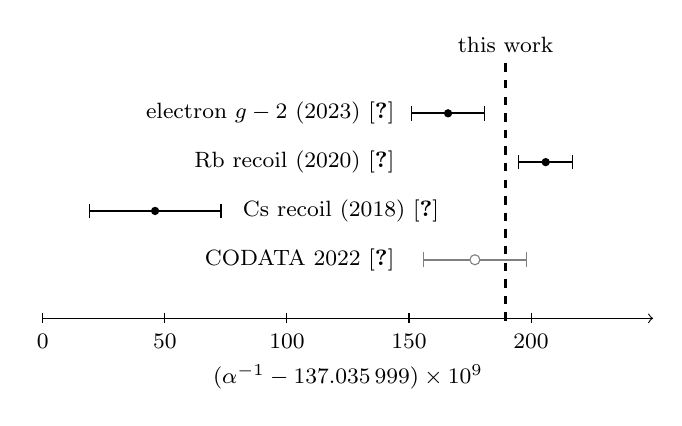
\begin{tikzpicture}[x=0.031cm, y=0.62cm, every node/.style={font=\footnotesize}]
\draw[->] (0,0) -- (250,0);
\foreach \t in {0,50,100,150,200} {\draw (\t,0.1) -- (\t,-0.1); \node[anchor=north] at (\t,-0.12) {$\t$};}
\node[anchor=north] at (125,-0.75) {$(\alpha^{-1} - 137.035\,999)\times 10^{9}$};
\draw[dashed, thick] (189.57,-0.05) -- (189.57,5.25);
\node[anchor=south] at (189.57,5.25) {this work};
\draw[thick] (151,4.2) -- (181,4.2); \draw (151,4.05) -- (151,4.35); \draw (181,4.05) -- (181,4.35); \fill (166,4.2) circle (1.5pt);
\node[anchor=east] at (148,4.2) {electron $g-2$ (2023) \cite{fan2023}};
\draw[thick] (195,3.2) -- (217,3.2); \draw (195,3.05) -- (195,3.35); \draw (217,3.05) -- (217,3.35); \fill (206,3.2) circle (1.5pt);
\node[anchor=east] at (148,3.2) {Rb recoil (2020) \cite{morel2020}};
\draw[thick] (19,2.2) -- (73,2.2); \draw (19,2.05) -- (19,2.35); \draw (73,2.05) -- (73,2.35); \fill (46,2.2) circle (1.5pt);
\node[anchor=west] at (78,2.2) {Cs recoil (2018) \cite{parker2018}};
\draw[thick, gray] (156,1.2) -- (198,1.2); \draw[gray] (156,1.05) -- (156,1.35); \draw[gray] (198,1.05) -- (198,1.35); \draw[gray, fill=white] (177,1.2) circle (1.8pt);
\node[anchor=east] at (148,1.2) {CODATA 2022 \cite{codata2022}};
\end{tikzpicture}
\caption{The inverse of the candidate of Eq.~(\ref{eq:alpha}), $\alpha_{\mathrm{cand}}^{-1} = 137.035\,999\,189\,6\ldots$ (dashed), against the one-standard-deviation intervals of the most precise determinations of $\alpha(0)$: the electron magnetic moment with the Standard Model prediction~\cite{fan2023}, $137.035\,999\,166(15)$; rubidium recoil~\cite{morel2020}, $137.035\,999\,206(11)$; cesium recoil~\cite{parker2018}, $137.035\,999\,046(27)$; and the CODATA 2022 adjustment of such inputs (open circle)~\cite{codata2022}, $137.035\,999\,177(21)$. The exact form carries no uncertainty of its own; it lies $+1.6\sigma$, $-1.5\sigma$, $+5.3\sigma$, and $+0.6\sigma$ from these values.}
\label{fig:comparison}
\end{figure}


\emph{Formalization.}---A single Lean~4 file, using only the core library and importing no results, builds the $172$ records from the slots and the commutator matrices, shows that each is an eigenvector of the exchange of the reads, applies the weight law, and evaluates Eq.~(\ref{eq:alpha}) exactly. Its main theorem has no hypotheses beyond the stated definitions, and its proof uses only propositional extensionality. The file's definitions, those of Table~\ref{tab:inputs}, are the axiom as a structure, its five definitions with the three clauses that decide the weights, and the two definitions of the computed quantity. The read cap enters only the theorems that select the link, as a named hypothesis citing the theorems of St{\o}rmer, Woronowicz, and Choi for the definition of a readable type, which the file does not formalize, and the Photon Conjecture does not appear. What it certifies is that the stated definitions produce Eq.~(\ref{eq:alpha}) exactly, with every count computed and no number entered by hand~\cite{SM}. It accompanies this Letter, with the record table and a script that rebuilds the records.

\emph{Discussion.}---A single quantum-information axiom with no adjustable parameters yields a number that agrees with the measured Thomson-limit fine-structure constant to ten significant figures, $0.6\sigma$ from the CODATA 2022 value. The number is computed from the axiom, its five definitions, and the two definitions of the computed quantity, the two-point function and the normalized readout, and nothing in it is fit to $\alpha$. The read cap, which the definition of fix yields with the theorems of St{\o}rmer, Woronowicz, and Choi, selects the link, three clauses of the definitions (that a read is an act at the end at which it is taken and reaches its far end whole, that the copies of a shared qudit are one qudit, and that the known holds under every exchange of reads or of pairs) decide the configuration and the weights, the on-shell definition names the result, and the conjecture identifies it. Table~\ref{tab:inputs} of the Supplemental Material lists every input and where it enters, and Sec.~\ref{sec:s-alternatives} lists every alternative that would change the number, these clauses worded otherwise among them, with the definition that excludes it without comparison with $\alpha$ and, where it is computed, its value, two of them within one percent of the computed value~\cite{SM}.

It is striking that an axiom about entangled pairs, which mentions neither charge nor spacetime, singles out the Standard Model gauge group and reaches $\alpha(0)$ at this precision. This is the first separately published result of Chain Theory, our broader program to study fundamental physics through the lens of quantum information. If the conjecture holds, $\alpha(0)$ is a weighted count over the $172$ measurement records of one entangled pair, and the premise that fundamental physics arises from networks of entangled pairs may prove a fertile avenue toward physics beyond the Standard Model.

\begin{acknowledgments}
\emph{Acknowledgments.}---The author thanks S. Guineau, J. Halverson, I. MacCormack, M. Pines, and A. Morari for helpful discussions. This work was developed as part of a long-term human-superintelligence collaboration supervised by the human author. It was assisted by resources of Physical Superintelligence PBC, in which the author has a financial interest.
\end{acknowledgments}

\begin{thebibliography}{99}
\bibitem{fan2023} X. Fan, T. G. Myers, B. A. D. Sukra, and G. Gabrielse, Phys. Rev. Lett. \textbf{130}, 071801 (2023).
\bibitem{morel2020} L. Morel, Z. Yao, P. Clad\'{e}, and S. Guellati-Kh\'{e}lifa, Nature \textbf{588}, 61 (2020).
\bibitem{parker2018} R. H. Parker, C. Yu, W. Zhong, B. Estey, and H. M\"{u}ller, Science \textbf{360}, 191 (2018).
\bibitem{codata2022} P. J. Mohr, D. B. Newell, B. N. Taylor, and E. Tiesinga, Rev. Mod. Phys. \textbf{97}, 025002 (2025).
\bibitem{wyler1969} A. Wyler, C. R. Acad. Sci. Paris A \textbf{269}, 743 (1969).
\bibitem{wyler1971} A. Wyler, C. R. Acad. Sci. Paris A \textbf{272}, 186 (1971).
\bibitem{robertson1971} B. Robertson, Phys. Rev. Lett. \textbf{27}, 1545 (1971).
\bibitem{gilmore1972} R. Gilmore, Phys. Rev. Lett. \textbf{28}, 462 (1972).
\bibitem{weinberg1964} S. Weinberg, Phys. Rev. \textbf{135}, B1049 (1964).
\bibitem{weinberg1965} S. Weinberg, Phys. Rev. \textbf{140}, B516 (1965).
\bibitem{peskin1995} M. E. Peskin and D. V. Schroeder, \textit{An Introduction to Quantum Field Theory} (Addison-Wesley, Reading, MA, 1995).
\bibitem{appelquist1975} T. Appelquist and J. Carazzone, Phys. Rev. D \textbf{11}, 2856 (1975).
\bibitem{bekenstein1981} J. D. Bekenstein, Phys. Rev. D \textbf{23}, 287 (1981).
\bibitem{thooft1993} G. 't Hooft, arXiv:gr-qc/9310026.
\bibitem{susskind1995} L. Susskind, J. Math. Phys. \textbf{36}, 6377 (1995).
\bibitem{hardy2001} L. Hardy, arXiv:quant-ph/0101012.
\bibitem{chiribella2011} G. Chiribella, G. M. D'Ariano, and P. Perinotti, Phys. Rev. A \textbf{84}, 012311 (2011).
\bibitem{jacobson1995} T. Jacobson, Phys. Rev. Lett. \textbf{75}, 1260 (1995).
\bibitem{vanraamsdonk2010} M. Van Raamsdonk, Gen. Relativ. Gravit. \textbf{42}, 2323 (2010).
\bibitem{horodecki1996} M. Horodecki, P. Horodecki, and R. Horodecki, Phys. Lett. A \textbf{223}, 1 (1996).
\bibitem{phorodecki1997} P. Horodecki, Phys. Lett. A \textbf{232}, 333 (1997).
\bibitem{horodecki1998} M. Horodecki, P. Horodecki, and R. Horodecki, Phys. Rev. Lett. \textbf{80}, 5239 (1998).
\bibitem{horodecki2009} R. Horodecki, P. Horodecki, M. Horodecki, and K. Horodecki, Rev. Mod. Phys. \textbf{81}, 865 (2009).
\bibitem{wheeler1990} J. A. Wheeler, in \textit{Complexity, Entropy, and the Physics of Information}, edited by W. H. Zurek (Addison-Wesley, Redwood City, CA, 1990), pp.~3--28.
\bibitem{verstraete2004} F. Verstraete and J. I. Cirac, arXiv:cond-mat/0407066.
\bibitem{bennett1996a} C. H. Bennett, G. Brassard, S. Popescu, B. Schumacher, J. A. Smolin, and W. K. Wootters, Phys. Rev. Lett. \textbf{76}, 722 (1996).
\bibitem{bennett1996b} C. H. Bennett, H. J. Bernstein, S. Popescu, and B. Schumacher, Phys. Rev. A \textbf{53}, 2046 (1996).
\bibitem{zukowski1993} M. \.{Z}ukowski, A. Zeilinger, M. A. Horne, and A. K. Ekert, Phys. Rev. Lett. \textbf{71}, 4287 (1993).
\bibitem{horowitz2004} G. T. Horowitz and J. Maldacena, J. High Energy Phys. \textbf{02} (2004) 008.
\bibitem{lloyd2011} S. Lloyd, L. Maccone, R. Garcia-Patron, V. Giovannetti, Y. Shikano, S. Pirandola, L. A. Rozema, A. Darabi, Y. Soudagar, L. K. Shalm, and A. M. Steinberg, Phys. Rev. Lett. \textbf{106}, 040403 (2011).
\bibitem{wootters1989} W. K. Wootters and B. D. Fields, Ann. Phys. (N.Y.) \textbf{191}, 363 (1989).
\bibitem{SM} See Supplemental Material below for the proofs, the configuration enumeration, the alternatives, the explicit matrices, and the formalization, which includes Refs.~\cite{gottesman2004,aaronson2005}.
\bibitem{zurek2003} W. H. Zurek, Phys. Rev. Lett. \textbf{90}, 120404 (2003).
\bibitem{horodecki1999} M. Horodecki and P. Horodecki, Phys. Rev. A \textbf{59}, 4206 (1999).
\bibitem{stormer1963} E. St{\o}rmer, Acta Math. \textbf{110}, 233 (1963).
\bibitem{woronowicz} S. L. Woronowicz, Rep. Math. Phys. \textbf{10}, 165 (1976).
\bibitem{choi1975} M.-D. Choi, Linear Algebra Appl. \textbf{12}, 95 (1975).
\bibitem{choi1975cp} M.-D. Choi, Linear Algebra Appl. \textbf{10}, 285 (1975).
\bibitem{jamiolkowski1972} A. Jamio{\l}kowski, Rep. Math. Phys. \textbf{3}, 275 (1972).
\bibitem{baez2010} J. Baez and J. Huerta, Bull. Am. Math. Soc. \textbf{47}, 483 (2010).
\bibitem{ollivier2004} H. Ollivier, D. Poulin, and W. H. Zurek, Phys. Rev. Lett. \textbf{93}, 220401 (2004).
\bibitem{zurek2009} W. H. Zurek, Nat. Phys. \textbf{5}, 181 (2009).
\bibitem{feynman1948} R. P. Feynman, Rev. Mod. Phys. \textbf{20}, 367 (1948).
\bibitem{gottesman2004} D. Gottesman and J. Preskill, J. High Energy Phys. \textbf{03} (2004) 026.
\bibitem{aaronson2005} S. Aaronson, Proc. R. Soc. A \textbf{461}, 3473 (2005).
\end{thebibliography}

\clearpage
\onecolumngrid
\begin{center}
\textbf{\large Supplemental Material}\\[4pt]
\textbf{A Parameter-Free Candidate for the Fine-Structure Constant from Entangled Qudits}
\end{center}
\bigskip

\setcounter{equation}{0}\renewcommand{\theequation}{S\arabic{equation}}\renewcommand{\theHequation}{S\arabic{equation}}
\setcounter{table}{0}\renewcommand{\thetable}{S\arabic{table}}\renewcommand{\theHtable}{S\arabic{table}}
\setcounter{figure}{0}\renewcommand{\thefigure}{S\arabic{figure}}\renewcommand{\theHfigure}{S\arabic{figure}}
\setcounter{theorem}{0}\renewcommand{\thetheorem}{S\arabic{theorem}}\renewcommand{\theHtheorem}{S\arabic{theorem}}
\setcounter{lemma}{0}\renewcommand{\thelemma}{S\arabic{lemma}}\renewcommand{\theHlemma}{S\arabic{lemma}}
\setcounter{corollary}{0}\renewcommand{\thecorollary}{S\arabic{corollary}}\renewcommand{\theHcorollary}{S\arabic{corollary}}
\setcounter{secnumdepth}{1}
\renewcommand{\thesection}{S\arabic{section}}
\def\UrlBreaks{\do\.\do\_}
\newcommand{\lean}[1]{\nolinkurl{#1}}

This Supplement gives the proofs behind the Letter: the model and its measurement theory (S1--S2), the charge and its conservation (S3--S4), the configuration and its readout dimension (S5--S6), the count of records and the value, also drawn in strands (S7), the on-shell correspondence (S8), the alternatives the derivation rules out (S9), the explicit matrices (S10), the formalization (S11), and a glossary (S12). Equations, theorems, figures, and the conjecture of the Letter are cited by their numbers there; those of this Supplement carry the prefix S. Table~\ref{tab:inputs} lists every input beyond the axiom and where it enters.

\begin{table}[h]
\caption{Every input beyond the axiom, and where it enters. Numbers in the last column without the prefix S are those of the Letter.}
\label{tab:inputs}
\footnotesize
\begin{ruledtabular}
\begin{tabular}{>{\raggedright\arraybackslash}p{0.36\linewidth}>{\raggedright\arraybackslash}p{0.33\linewidth}>{\raggedright\arraybackslash}p{0.21\linewidth}}
input & status & enters \\ \hline
five definitions & the axiom's terms spelled out; their properties are Corollaries~\ref{cor:s-qudit}--\ref{cor:s-single} & throughout \\
a read fixes two ends only when every positive map between them is decomposable & the definition of fix: certainty leaves nothing open & the read cap \\
St{\o}rmer, Woronowicz, Choi; Horodecki & theorems of the literature & the cap is $d_{1}d_{2}\leq 6$; the dark sector is undistillable \\
a read is an act at the end at which it is taken and reaches its far end whole, hence the end rule & clause of the definition of a read & Theorem~\ref{thm:object}, Eq.~(\ref{eq:gain}) \\
the copies of a shared qudit are one qudit, so an exchange of its pairs moves only their far ends & clause of the definition of sharing & Eq.~(\ref{eq:gain}) \\
the known holds under every exchange of reads or of pairs, so a record survives an exchange that returns it times its own sign & clause of the definition of the known & Eq.~(\ref{eq:gain}) \\
a record: two letters, the two insertions; weight $\sqrt{k_{r}}$, not $k_{r}$ & step of the model & Eq.~(\ref{eq:alpha}) \\
units: $\openone_{R}$ reads one; $\mathcal{Q}$ read at the ket side & definition of the computed quantity, after the on-shell scheme & Eqs.~(\ref{eq:readout}), (\ref{eq:alpha}) \\
no failure branch of a distillation, a postselection in a laboratory & step of the model, from the axiom & the joint state, Sec.~\ref{sec:s-count} \\
two-point function: two reads, one unread link & definition of the computed quantity, after the on-shell scheme & Theorem~\ref{thm:object}, Eq.~(\ref{eq:N}) \\
on-shell correspondence of Eq.~(\ref{eq:readout}) & one definition & names Theorem~\ref{thm:value} \\
Photon Conjecture & conjecture & identification with $\alpha(0)$ \\
\end{tabular}
\end{ruledtabular}
\end{table}

\section{The model}
\label{sec:s-model}

The axiom reads: \textit{Nothing exists but finitely many maximally entangled pairs of qudits, some qudits shared, known only by distilling them.} Its five definitions (qudit, shared, distilling, read, known) spell out its terms, and the properties of each that the Letter uses follow from it as the corollaries below. Lemma~\ref{lem:s-matching} supplies the matchings used in the first.

\begin{corollary}[A qudit]
\label{cor:s-qudit}
The state space of an end is the span of the outputs of the acts on it, the pair kets under the admissible matchings. At the qutrit--qubit link that span is the whole six-dimensional tensor space. The moduli of its inner products are fixed by the Born readout; their phases beyond the moduli are fixed by no readout.
\end{corollary}
\begin{proof}
The acts on an end are distillations, whose outputs are pair kets on the common support, carried by the matchings over the orbit of the pair ket. At $(2,3)$ the orbit under the fourth-root matchings at both ends has $96$ vectors and spans all $6$ dimensions, as does the cyclic module generated from the pair ket by the matrix units of the two ends; the same holds at every type with ends of dimension two to four. The frame operator of the orbit is a scalar, so the Born readouts, the squared moduli of the Gram elements at all $576$ pairs of the frame, fix the moduli of the inner products. The remaining phases are moved by matchings that fix every readout.
\end{proof}

A pair of the axiom of type $(d_{1},d_{2})$, also called a \emph{link}, joins two qudits of dimensions $d_{1},d_{2}$ in the pair ket on their common support, and distilling two qudits outputs the pair of their type. A qudit is \emph{shared} when it is one end of two or more pairs, spelling out ``some qudits shared'', and its copies, one per pair, are one qudit, so an exchange of its pairs leaves it in place and moves only their far ends.

\begin{corollary}[Distilling]
\label{cor:s-distill}
An act on two qudits whose output is a pair of the two on their common support is exactly the projection $P_{m}$ onto a maximally entangled pair there.
\end{corollary}
\begin{proof}
Nothing exists but maximally entangled pairs, so an act on two qudits leaves them in a pair or in nothing. A unitary preserves the purity of its input and makes no pair; a local measurement, or a label of one, leaves no pure state; a replacement channel leaves the partners in no pair; a sub-maximal projection reaches no configuration of the axiom. The rank of every operator equals the Schmidt rank of its output across the cut, and $P_{m}$ returns the pair, so the act is $P_{m}$ and nothing else.
\end{proof}

\begin{corollary}[A read]
\label{cor:s-read}
(i) A read, a distillation of the two ends of a pair in a basis of one end, one read per basis, has at most $d+1$ bases at an end of dimension $d$: the mutually unbiased eigenbases of the clock and shift operators~\cite{wootters1989}, three at $d=2$ and four at $d=3$. (ii) The basis a read gives its qudit is the label it attaches beyond the projection and passes along the pair. (iii) At each element of its basis, the read determines the state of the far end with no freedom. (iv) The basis a read passes reaches the far end whole, so a read is taken at the larger end of a pair, or at either end of an equal one.
\end{corollary}
\begin{proof}
For (iii), $\bra{e_{i}}\omega\rangle\propto\overline{\ket{e_{i}}}$ transported to the far end, by the transpose identity $(A\otimes\openone)\ket{\omega}=(\openone\otimes A^{T})\ket{\omega}$ at every matrix unit of the support. At the qutrit--qubit link the far direction is determined at all four bases of the qutrit, $152$ of $152$ matrix elements, with no sign left free. These far-end states need not form an orthonormal basis of the far end: a qutrit basis gives three qubit states, one of them zero when a basis vector lies outside the common support. For (iv), the far-end states lie in the common support and span it, which is the whole far end exactly when the far end is no larger than the end at which the read is taken.
\end{proof}

\begin{corollary}[The known and the commutator records]
\label{cor:s-known}
What is known of a qudit is what its reads fix jointly, under every matching of its pairs and every exchange of its reads or of its pairs. To \emph{fix} is to determine with certainty on the one copy (Corollary~\ref{cor:s-single}), and certainty leaves nothing open: no expectation value is estimated anywhere, and a read fixes two ends only when every consistent relation between them is of a kind distillations carry (Sec.~\ref{sec:s-read}). Two reads that anticommute therefore fix a further record, their product, with their order as its sign.
\end{corollary}
\begin{proof}
The first clause restates the axiom (``known only by distilling'') with the definition of a read. For the second, two reads $A$ and $B$ compose to $AB=\tfrac12\{A,B\}+\tfrac12[A,B]$, the first part fixed whatever their order and the second by it. When they anticommute the first part vanishes, and the composite is fixed by the two reads with their order as its sign. The letters of two of the bases of Corollary~\ref{cor:s-read}(i) are the clock and shift operators, whose commutator phase is a primitive $d$-th root of unity. At the qubit end it is $-1$ for all three pairs of bases, so two reads there compose in their two orders to one further operator with the order as its sign. That operator is traceless, outside the span of the identity and the two reads, and fixed under every matching, so it is a record by the first clause. Only a sign can play this role. For two invertible reads with $AB=\lambda BA$ at an end of dimension $d$, determinants give $\lambda^{d}=1$, and reversing the order multiplies the composite by $\lambda^{-1}$ one way and by $\lambda$ the other, so the order labels it, as an eigenvalue of exchanging the two reads, an involution, only if $\lambda=\lambda^{-1}$. Together $\lambda^{\gcd(d,2)}=1$: a sign is possible only at even $d$, which the qubit's reads realize, and at the qutrit no two reads anticommute, their Weyl phase being a cube root of unity, which is not its own inverse.
\end{proof}

\begin{corollary}[A single copy]
\label{cor:s-single}
No link between the same two qudits exists twice, and no act makes one, so a read acts once on the one copy of the link it reads.
\end{corollary}
\begin{proof}
The pairs are finitely many states of the named qudits, and distilling, the one act, projects existing qudits and creates none. A second link between the same two qudits in the same state would be a further entry of the pair list at the same named qudits, which no act produces. Statistics over fresh instances of one link, and a repeated read of one link on a fresh copy, are therefore unavailable. Distinct links in the same state at distinct qudits, such as the three links of the object, are not excluded.
\end{proof}

\begin{lemma}[The matching group]
\label{lem:s-matching}
The matchings of an end of dimension $d$ admitted by the definition of the known are exactly the unitaries $U$ of its support, acting on a pair as $U\otimes\bar{U}$. The monomial matrices with fourth-root-of-unity entries form a finite subgroup $G_{d}$ of order $d!\,4^{d}$: $32$ at $d=2$ and $384$ at $d=3$.
\end{lemma}
\begin{proof}
A matching carries an orthonormal basis of the support to an orthonormal basis, in any order and with any phase a read cannot see, so it is a unitary of the support, and every unitary arises this way. By the transpose identity $U$ at the near end acts as $\bar{U}$ at the far end, and $U\otimes\bar{U}$ fixes $\ket{\omega_{m}}$. The phases whose squares are the signs of Corollary~\ref{cor:s-known} are the fourth roots of unity.
\end{proof}

\begin{theorem}[The pair ket and the amplitude level]
\label{thm:s-pairket}
$\ket{\omega_{d}}$ is the unique pure state fixed by the isotropic twirl $T_{d}(A)=\int dU\,(U\otimes\bar{U})A(U\otimes\bar{U})^{\dagger}$. Its components in the $d$ matched directions are $1/\sqrt{d}$, the square roots of the Born readouts $1/d$, so a read is read at the amplitude level. Two distillations at a shared qudit compose to the pair ket on their common support.
\end{theorem}
\begin{proof}
$U\mapsto U\otimes\bar{U}$ decomposes into the trivial representation on $\ket{\omega_{d}}$ and the adjoint on its complement, two inequivalent irreducibles, so the fixed-point algebra is spanned by $\openone$ and $P_{d}$, with minimal projections of ranks $1$ and $d^{2}-1\geq 3$. Under $G_{d}$ alone the fixed-point algebra is three-dimensional, and at $d=2$ the state $(\ket{11}-\ket{22})/\sqrt{2}$ is also fixed, so uniqueness uses the whole group. Summing over the $d$ matched directions, the trace of the amplitudes is $d\cdot(1/\sqrt{d})=\sqrt{d}$ and the trace of the readouts is $d\cdot(1/d)=1$. These differ at every $d>1$, so the root is taken ahead of the sum over the matched directions. For two pairs $\ket{\omega}_{AB}$ and $\ket{\omega}_{BC}$, the product of the two rank-one projections yields $\ket{\omega}_{AC}$ on the common support.
\end{proof}

\textbf{The Born square.} Every act is a projection whose complement is no state of the model (Corollary~\ref{cor:s-distill}), so no act has a branch whose probability the Born rule would give. The Born square enters as a readout weight, the number a projection delivers on the one copy, never a frequency over outcomes: the bare transmission is the Born square of the pair ket at its two matched directions, and the amplitudes $1/\sqrt{d}$ of Theorem~\ref{thm:s-pairket} are amplitudes of the one state.

\textbf{Distillation and postselection.} Between two pairs the act is the projection at the heart of entanglement swapping~\cite{zukowski1993}. With qudits $1$--$2$ and $3$--$4$ in pairs of dimension $d$, the partial inner product on qudits $2$ and $3$ is
\begin{equation}
\bra{\omega_{d}}_{23}\,\ket{\omega_{d}}_{12}\ket{\omega_{d}}_{34}=\frac{1}{d}\,\ket{\omega_{d}}_{14},
\label{eq:s-swap}
\end{equation}
each of the $d$ terms of the result a product of three pair amplitudes, $d^{-3/2}$. In a laboratory, $P_{d}$ on qudits $2$ and $3$ is one outcome of a Bell measurement, obtained with probability $1/d^{2}$, and the swapping protocol uses all $d^{2}$ outcomes: it sends the one obtained and corrects qudit $1$ or $4$. The model keeps the projection and not the protocol. Its complement is no configuration of the axiom (Corollary~\ref{cor:s-distill}), so the act has no other outcome, sends nothing, and corrects nothing. It leaves $2$--$3$ and $1$--$4$ in pairs where $1$--$2$ and $3$--$4$ were: entanglement is moved and none is added. Between links of unequal dimension the bookkeeping differs: the join of Sec.~\ref{sec:s-count} takes two qutrit--qubit links to the qutrit pair $\ket{\omega_{3}}$ of the read copies and the qubit pair $\ket{\omega_{2}}$ of the read qubits. In laboratory terms the act is a postselection, and the factor $\sqrt{6}$ of the joint state there normalizes the postselected state. Postselection has been proposed as a law before, as a final state at the black-hole singularity~\cite{horowitz2004}, to which there are known objections~\cite{gottesman2004}, and as a model of closed timelike curves~\cite{lloyd2011}; as a resource it is strong, since postselected polynomial-time quantum computation is the class PP~\cite{aaronson2005}. Such laws are in general nonlinear, because the normalization depends on the input. In our model, every input of a distillation is a configuration of pairs, fixed under every matching, so its normalization is one fixed number, $\sqrt{6}$ at the object. That a failed projection has nowhere to leave its qudits follows from ``nothing exists but \ldots\ pairs'': there is no state outside the pairs. Whether a postselected law of this kind is consistent with the rest of physics is not settled here; the derivation uses it where Table~\ref{tab:inputs} lists it.

\textbf{The shared qudit as copies.} A pure maximally entangled pair has product marginals with every third system, so a qudit at the end of $k$ links is carried as $k$ copies of itself, one per link. The copies at read links are contracted by the reads, whose composition at the shared qudit is the join, a unitary on the composed support (Lemma~\ref{lem:s-join}); the copy at an unread link is contracted with nothing and carries the state through its connected part alone. Monogamy is never violated: each link is maximally entangled with its own copy, as in a projected entangled pair state. These copies of a shared qudit, one per link, are distinct from the copies of a link excluded by Corollary~\ref{cor:s-single}.

\begin{lemma}[The join is unitary]
\label{lem:s-join}
A pure pair on a common support of rank $m$ has a flat reduced state exactly when its coefficient matrix is a multiple of a unitary on the support. The pair ket is flat in every dimension, so the join of two links at a shared qudit, the contraction of their coefficient matrices at the shared index, is a unitary on the composed support.
\end{lemma}
\begin{proof}
By the Schmidt decomposition, flatness says the $m$ nonzero Schmidt coefficients are equal; the coefficient matrix is then a scaled partial isometry of rank $m$, and a product of two such is again one.
\end{proof}

\section{What a read can measure}
\label{sec:s-read}

\begin{lemma}[The commutant]
\label{lem:s-commutant}
On $\mathbb{C}^{d}\otimes\mathbb{C}^{d}$ the commutant of $\{U\otimes\bar{U}:U\in G_{d}\}$ is spanned by $\openone$, $P_{d}$, and the diagonal projector $D_{d}=\sum_{i}\ket{ii}\!\bra{ii}$; under the full unitary group it is spanned by $\openone$ and $P_{d}$ alone~\cite{horodecki1999}.
\end{lemma}
\begin{proof}
Write $A=\sum a_{ij,kl}\ket{ij}\!\bra{kl}$. A diagonal element $\mathrm{diag}(\phi_{1},\ldots,\phi_{d})$ multiplies $a_{ij,kl}$ by $\phi_{i}\bar{\phi}_{j}\bar{\phi}_{k}\phi_{l}$. Since each $\phi_{m}$ ranges independently over the fourth roots of unity, $A$ is fixed exactly when the net exponent at every direction vanishes, which leaves $\ket{ii}\!\bra{kk}$ and $\ket{ij}\!\bra{ij}$. The permutations have three orbits on these, with sums $D_{d}$, $dP_{d}-D_{d}$, and $\openone-D_{d}$, which span the same space as $\openone$, $P_{d}$, and $D_{d}$. The character formula $|G_{d}|^{-1}\sum_{U}|\tr U|^{4}=3$ at $d=2,3,4$ confirms the dimension. Under the full group, Schur's lemma leaves $\openone$ and $P_{d}$.
\end{proof}

\begin{theorem}[The unique readout]
\label{thm:s-readout}
With the identity of $R$ as the unit of the readout, every readout a read of a configuration can deliver is the normalized trace $\tr_{R}M/\dim R$ of its dressed insertion $M$, an operator on the readout algebra $R$, Eq.~(\ref{eq:readout}) of the Letter. At the bare insertion, the identity of $R$, it is one.
\end{theorem}
\begin{proof}
A readout is a trace against an element of $R$ invariant under every matching, so that element lies in the span of $\openone$, $P$, and $D$ at each end (Lemma~\ref{lem:s-commutant}). A read is a projection onto a pair, and every pair projector a read delivers is $P$ itself, so $D$ lies outside what reads deliver: on the vacuum $D$ reads like the identity, yet it differs from it as an operator, so the exclusion comes from the definition of a read and not from an expectation value. Which invariant element sets the unit is a definition. The commutant allows two at a read link, $\openone$ and $P$, and the model uses both at different factors: the identity of $R$ is the unit of the trace functional, the denominator of $Z_{3}$, and $P$ gives the certain transmission $\tfrac{1}{2}+\tfrac{1}{2}$ of the bare link, $\alpha_{\mathrm{bare}}=1$ (Sec.~\ref{sec:s-onshell}). With the identity of $R$ as the unit, the readout is $\tr_{R}(\cdot)/\dim R$. The trace is invariant under every matching, so an insertion and its twirl give the same readout.
\end{proof}

\textbf{No state of the model is bound entangled.} A read meets pair kets, pure and maximally entangled, so its projection onto the pair succeeds with probability one on the single copy (Corollary~\ref{cor:s-single}). That certainty is the bare unit $\tfrac{1}{2}+\tfrac{1}{2}$ of Sec.~\ref{sec:s-onshell}. No expectation value, of a witness or of anything else, is estimated anywhere. Every link is a pure maximally entangled state, distillable in every dimension, and two qudits that share no link are uncorrelated (the copies of Sec.~\ref{sec:s-model}). What a single read can fail to fix is therefore not a state but a relation between the two ends of a type, the way the reads relate their operator algebras.

\begin{lemma}[What reads carry]
\label{lem:s-carry}
A linear map $\Lambda:M_{d_{1}}\to M_{d_{2}}$ is \emph{decomposable} if $\Lambda=\Phi_{1}+\Phi_{2}\circ T$ with $\Phi_{1},\Phi_{2}$ completely positive and $T$ the transpose. Every map between the two ends of a link that reads compose, by composition and by taking reads jointly, is decomposable.
\end{lemma}
\begin{proof}
A read acts at its own end by the projection onto its pair and by the matchings $U\otimes\bar{U}$, which are completely positive, and carries an operator to the far end by the transpose identity $(A\otimes\openone)\ket{\omega}=(\openone\otimes A^{T})\ket{\omega}$, which is $T$ on the support. For $\Phi$ completely positive with Kraus operators $K$, $T\circ\Phi\circ T$ has Kraus operators $\bar{K}$ and is completely positive, and $T\circ T$ is the identity. So every composite is completely positive or completely positive after $T$, and reads taken jointly add such maps.
\end{proof}

\textbf{Certainty at the ends of a pair.} A positive map between the operator algebras of two ends is a consistent way of relating them: it carries every description of one end, a positive operator, to a description of the other, and the matchings are its unitary cases. Reads carry only maps of the decomposable kinds (Lemma~\ref{lem:s-carry}). A type is \emph{readable} when every positive map between its ends is decomposable and \emph{dark} otherwise. To fix is to determine with certainty, and certainty leaves nothing open: \emph{a read fixes two ends only when every consistent relation between them is of a kind distillations carry}, since a relation of another kind would leave open how one end describes the other. At a qudit the relations the pair state leaves free are the matchings, all of a kind reads carry, and the known is what the reads fix under every one of them and under every exchange of reads or of pairs (Corollary~\ref{cor:s-known}). At the ends of a pair the clause ranges over every consistent relation between them, not only over the matchings, and a relation of a kind no distillation carries is one the ends admit and no distillation could fix. The positive maps between two ends depend only on their dimensions, and so does readability, so a single read fixes the ends of a pair exactly when its type is readable. Under a weaker definition of fix, blind to the relations between ends, the read cap below would be a premise rather than a consequence.

\textbf{Where the cap sits.} Every positive map is decomposable at $(2,2)$~\cite{stormer1963} and at $(2,3)$ and $(3,2)$~\cite{woronowicz}. Non-decomposable positive maps exist at $(2,4)$~\cite{woronowicz} and at $(3,3)$~\cite{choi1975}, Choi's map, and compressing to a subspace and embedding carry them to every type with $d_{1}d_{2}\geq 8$. No product of two integers $\geq 2$ equals seven. So a type of dimensions $d_{1},d_{2}\geq 2$ is readable, and a single read fixes its ends, if and only if $d_{1}d_{2}\leq 6$: the \emph{read cap}, the form in which the Letter and the Lean file use it. A dark type's links stay maximally entangled and distillable; what no distillation carries is a relation between their ends, not a state.

\textbf{Why dark is undistillable.} Under the Choi--Jamio{\l}kowski correspondence~\cite{choi1975cp,jamiolkowski1972} positive maps are entanglement witnesses, and decomposable maps are the witnesses $A+B^{T_{2}}$ with $A,B\geq 0$~\cite{horodecki1996,horodecki2009}. At $(2,2)$ and $(2,3)$ these decide entanglement for every state of the type~\cite{horodecki1996}. At $d_{1}d_{2}\geq 8$ the maps that reads cannot carry detect entangled states with positive partial transpose~\cite{phorodecki1997}, from which no number of copies distills a pair~\cite{horodecki1998}. A dark type therefore has a sector that standard distillation never reaches, though each of its links is maximally entangled; the cap concerns that sector of the type, not the link's own state.

\begin{lemma}[The readable types]
\label{lem:s-readrule}
The readable types are $(2,2)$ and $(2,3)$, and $(2,3)$ is the only one with unequal ends.
\end{lemma}
\begin{proof}
By the read cap a type is readable exactly when $d_{1}d_{2}\leq 6$. If $d_{1}\geq 4$ then $d_{1}d_{2}\geq 8$, so both dimensions are at most $3$, and of $(2,2)$, $(2,3)$, and $(3,3)$ only the first two have product at most six.
\end{proof}

\textbf{Remark: the readers.} A second route reaches the same cap, with every link maximally entangled throughout, under one further premise. (i) A read spans an end only if the end's dimension is at most the reader's, the computation behind the end rule (\lean{fixesFar_iff_le}); with the qubit and the qutrit as the readers, no end of dimension $4$ or more is spanned. (ii) A read reaches its far end by the transpose identity, under which the far end transforms by $\bar{U}$ where its partner transforms by $U$. The premise is that the far end holds the passed basis as a basis of its own, so that a matching at the far end undoes the conjugation, $V\bar{U}V^{\dagger}\propto U$ for every matching $U$. At a qubit $\sigma_{y}$ does, $\sigma_{y}\bar{U}\sigma_{y}=(\det\bar{U})\,U$, and on traceless letters $A^{T}=-\sigma_{y}A\sigma_{y}$ (\lean{qubit_absorbs_conjugation}). At a qutrit no unitary does, since the defining representation of $SU(3)$ is inequivalent to its conjugate; on the matching group, $U=\mathrm{diag}(i,1,1)$ already has $(\tr\bar{U})^{2}\neq(\tr U)^{2}$ with $\tr\bar{U}^{2}=\tr U^{2}\neq 0$, which no $V\bar{U}V^{\dagger}=cU$ allows (\lean{qutrit_conjugation_obstruction}). So the far end of a read is a qubit. Together, $(2,2)$ is readable, $(2,3)$ is readable at its qutrit end, $(3,3)$ is dark because its far end is a qutrit whichever end is read, and every type with an end of dimension $4$ or more is dark: exactly the types with $d_{1}d_{2}\geq 8$ (\lean{readers_reproduce_the_cap}). The premise goes beyond the definition of the known, which the transpose itself satisfies at every dimension, $(UAU^{\dagger})^{T}=\bar{U}A^{T}U^{T}$, so this route is a second one and not the one the Letter takes; it also gives the end rule a second reason, since a $(2,3)$ link read at its qubit would have the qutrit as its far end. The selection of the link is the same under the readers and under the cap (\lean{reads_satisfy_the_read_cap}).

\section{The identification algebra and the acting charge}
\label{sec:s-charge}

The identification algebra of a link of type $(d_{1},d_{2})$ is $su(d_{1})\oplus su(d_{2})\oplus u(1)$: the block-diagonal traceless anti-Hermitian operators on $\mathbb{C}^{d_{1}}\oplus\mathbb{C}^{d_{2}}$, equivalently $s(u(d_{1})\oplus u(d_{2}))$, the infinitesimal basis changes at the two ends. An element $\xi=\xi_{1}\oplus\xi_{2}$ acts on the pair over the matched directions as $\xi_{1}\otimes\openone+\openone\otimes\xi_{2}$. At $(2,3)$ it has dimension $12$, and it is the Lie algebra of $S(U(3)\times U(2))\cong(SU(3)\times SU(2)\times U(1))/\mathbb{Z}_{6}$, the subgroup of $SU(5)$ preserving the splitting $\mathbb{C}^{2}\oplus\mathbb{C}^{3}$~\cite{baez2010}. Under it the tensor space $\mathbb{C}^{2}\otimes\mathbb{C}^{3}$ of the link carries the representation $(3,2)$ with hypercharge $Y=1/6$, on which $\mathcal{Q}=6iY$ acts as $i$: the quantum numbers of the left-handed quark doublet. Its explicit basis is in Sec.~\ref{sec:s-matrices}.

\begin{lemma}[The acting center]
\label{lem:s-center}
The center of the identification algebra is one-dimensional, spanned by $\mathcal{Q}=i\,\mathrm{diag}(d_{2}\openone_{d_{1}};\,-d_{1}\openone_{d_{2}})$, which acts on the whole link, the pair ket included, as the scalar $i(d_{2}-d_{1})$. Of the readable types only $(2,3)$ has a central generator that acts on its pair, $\mathcal{Q}=i\,\mathrm{diag}(3,3;\,-2,-2,-2)=6iY$, with $Y=\mathrm{diag}(\tfrac{1}{2},\tfrac{1}{2};\,-\tfrac{1}{3},-\tfrac{1}{3},-\tfrac{1}{3})$ the hypercharge generator of the embedding in $SU(5)$.
\end{lemma}
\begin{proof}
An element commuting with both ideals is a scalar on each block, $(x\openone_{d_{1}},y\openone_{d_{2}})$, and tracelessness gives $d_{1}x+d_{2}y=0$. On a matched direction it acts as $i(x+y)=i(d_{2}-d_{1})$, which vanishes exactly when $d_{1}=d_{2}$.
\end{proof}

\begin{theorem}[The stabilizer of the pair ket]
\label{thm:s-stabilizer}
At $(2,3)$ the elements of the identification algebra annihilating the pair ket form a subalgebra of dimension four, the null space of an action of rank eight. It is the direct sum of a diagonal $su(2)$, the elements $\zeta\oplus\bar{\zeta}$ with $\zeta$ on the qubit and $\bar{\zeta}$ on the two-dimensional common support of the qutrit, spanned by $e_{1}+e_{4}$, $e_{2}-e_{7}$, and $e_{3}-e_{10}$, and one further line. Its center is one line, at the unbroken generator $\mathcal{U}=i\,\mathrm{diag}(1,1;\,-1,-1,0)$, with the third qutrit level fixed at zero. $\mathcal{Q}$ reads $i$ on the pair ket, where $\mathcal{U}$ reads $0$. Of the $12288$ pairs of the finite joint matching group $G_{2}\times G_{3}$, $128$ fix the pair ket.
\end{theorem}
\begin{proof}
The condition that $\xi_{1}\oplus\xi_{2}$ annihilate $\ket{\omega_{2}}=(\ket{11}+\ket{22})/\sqrt{2}$ is a linear system of rank $8$ on the $12$ coordinates. Its four-dimensional null space and the center of the resulting subalgebra are written out in Sec.~\ref{sec:s-matrices}.
\end{proof}

\section{Conservation and the Ward identity}
\label{sec:s-ward}

The open ends of a configuration are counted by type: a ket end $+1$ and a bra end $-1$, at each end dimension.

\begin{lemma}[The conserved count]
\label{lem:s-conserved}
A functional of the open ends that is invariant under every matching and sees no global phase of a pair is, at $(2,3)$, a multiple of the count of $\mathcal{Q}$; at $(2,2)$ it is zero. The count is conserved at every read and every join, and the dressed two-point function of $\mathcal{Q}$ equals its bare one, $Z_{2}/Z_{1}=1$.
\end{lemma}
\begin{proof}
Matchings permute the directions of each end, so an invariant functional is constant on the directions of each end: $x$ on the qubit end and $y$ on the qutrit end. A read sees no global phase of a pair, which gives $2x+3y=0$ at $(2,3)$, so $(x,y)\propto(3,-2)$, the scalars of $\mathcal{Q}$; at $(2,2)$ it gives $4x=0$. The condition is the tracelessness of $\mathcal{Q}$, and the same scalars act on the pair ket, seen on a different space. On the full space of the two ends the count sums over all $d_{1}+d_{2}$ directions and is zero. On the link every vector pairs one direction of each end, so $\mathcal{Q}$ acts on the whole tensor space, the pair ket included, as the matched sum $i(x+y)=i(d_{2}-d_{1})=i$, nonzero at unequal ends (Lemma~\ref{lem:s-center}). The pair ket is charged although $\mathcal{Q}$ is traceless because the link matches one direction per end while the trace counts them all. A read adds one ket end and one bra end of one dimension and a join removes one of each, so the count changes by matched ket--bra pairs only. The twirl fixes $\mathcal{Q}$, so its insertion is unchanged by dressing at every matching; both factors are $-6$ at the bare unit. Under conjugation every operator with both ends in the link counts zero, $[\mathcal{Q},A]=0$; the unit of that count is the charge of one ket end, $i$ (Lemma~\ref{lem:s-unit}).
\end{proof}

\begin{theorem}[The Ward identity and the dressing per unit]
\label{thm:s-ward}
Let $W$ assign one weight to each end dimension, acting on the typed count of open ends. The vertex dressing by $W$, the count of $W$ at the subdivision of a dressed link, and the line count of $W$ through the undivided link coincide at every record exactly when $W$ is the same at every end dimension. The identity holds at the unit functional $W=(1,1,1)$ at all $48$ orderings of the subdivision and all $172$ records, and fails for $\mathcal{Q}$ and $\mathcal{U}$ read as one-end weights, $(6,-6,0)$ and $(2,-2,0)$. Per unit of the conserved count, the dressed weights of the $172$ records, each taken once, sum to the numerator of Eq.~(\ref{eq:alpha}) of the Letter, the ratio one. Counting read ends record by record instead (two at $168$ records, one at the three commutators, none at one record) gives the different element $(158+96\sqrt{2}+82\sqrt{3}+3\sqrt{6})/31104$, which is not a coupling per unit of the conserved count.
\end{theorem}
\begin{proof}
The vertex dressing differs from the count by the sum over link pairs of $W_{\mathrm{ket}}-W_{\mathrm{bra}}$, which vanishes on every configuration exactly when $W$ is the same at every end dimension present. Subdividing a dressed link at its read ends is one read and three joins, creating two new link pairs and one born pair; their contributions telescope to that of the undivided link. For $\mathcal{Q}$ the vertex and the count differ by the line of the link, $-24$ against $-12$. The unit functional reads $1$ at each of the four slots of the two reads, so every record carries one unit at the sector level and enters once.
\end{proof}

\section{The configuration}
\label{sec:s-config}

A configuration is a shared center of dimension $c\in\{2,3\}$ with a multiset of arms, each a link from the center to a far end of dimension $e\in\{2,3\}$, marked read or unread. A read arm is read at the center and passes its basis to the far end. The reads lie between $1$ and the basis bound $c+1$ of Corollary~\ref{cor:s-read}(i), and for the enumeration the links are bounded in the same way, between $2$ and $c+1$, with the unread links between $0$ and that bound. Theorem~\ref{thm:object} of the Letter does not depend on the bound on links, since a two-point function has exactly three links. Its readout dimension is the product over arms of the whole operator space $(ce)^{2}$ at a read arm and the traceless part $(c^{2}-1)(e^{2}-1)$ at an unread arm.

\begin{theorem}[The configurations under the derived bounds]
\label{thm:s-config}
There are $76$ configurations, $23$ at a qubit center and $53$ at a qutrit center; $42$ are admitted by the read cap. A configuration is readable when it has at least two reads, every read arm is of a readable type, the reads and links are within the bound, and every pair of read arms has a non-empty record space. Exactly $23$ configurations are readable (Table~\ref{tab:s-configs}).
\end{theorem}
\begin{proof}
Enumeration of the $76$ configurations under the stated bounds.
\end{proof}

Minimality does not select the object. The least readout dimension, $256$, belongs to a shared qubit with two $(2,2)$ reads, $57$ records, and the readout $(30+30\sqrt{2})/256$ under the same weight law; but $(2,2)$ carries no acting charge (Lemma~\ref{lem:s-center}), so this configuration fails the acting charge of Theorem~\ref{thm:object} of the Letter. The object stands at $31104$, tied for thirteenth of the $23$ by readout dimension with a shared qubit carrying two $(2,3)$ reads and one $(2,3)$ unread link, which has $174$ records. The two differ in which end is shared. With the links at the bound, the readable set has $16$ configurations and does not contain the object, which has three links under a bound of four. Three conditions select the object, the end rule (a), the two-point function (b), and an acting central charge on every link (Lemma~\ref{lem:s-center}), and none refers to $\alpha$ or to the Gram matrix.

\emph{(a) The end rule.} A read is an act at the end at which it is taken. By Corollary~\ref{cor:s-read}(iii) a qutrit-end read determines the qubit's state at every basis element with no freedom, at $152$ of $152$ matrix elements. A qubit-end read reaches the qutrit only on the two-dimensional common support, and the third qutrit direction is fixed by no read; it is the direction the unbroken generator $\mathcal{U}$ leaves at zero (Theorem~\ref{thm:s-stabilizer}). A read reaches its far end whole (Corollary~\ref{cor:s-read}(iv)), so only a qutrit-end read is a read of a $(2,3)$ link. So a $(2,3)$ link is read at its qutrit end, and a configuration that reads $(2,3)$ links has a qutrit center.

\emph{(b) The two-point function.} A two-point function has two insertions on one state. In our model, the two insertions are two reads of the link, and the state is the link itself, a third link of the same type at the same center, carried unread: reading it would be a third insertion. So a configuration of the two-point function has exactly two read arms and one unread arm, all three of one type. This is the model's definition of a two-point function. It selects the configuration whose readout is computed, and the on-shell identification of Sec.~\ref{sec:s-onshell} names the result.

Applied to Table~\ref{tab:s-configs}: the nine configurations that read a $(2,3)$ link at a qubit center fail (a). The nine qutrit-center configurations other than the object fail (b), having no unread link, more than two reads, or an unread link beyond the one of the link's type. Of the four at a qubit center with only $(2,2)$ reads, three fail (b), and the fourth, $2$R $2$R $2$U, satisfies (a) and (b) but carries no acting charge. The object is the only configuration that satisfies (a), (b), and the acting charge, which is Theorem~\ref{thm:object} of the Letter, and the values of the others are therefore not needed.

\begin{table}[h]
\caption{The $23$ configurations readable: center dimension, arms (far dimension; R read, U unread), counts of links, reads, and unread links, readout dimension, records per pair of read arms, and the far dimensions of the read arms. The object is marked $\star$.}
\label{tab:s-configs}
\begin{ruledtabular}
\begin{tabular}{clcccrrl}
center & arms & links & reads & unread & readout dimension & records & far ends of the read arms \\ \hline
2 & 2R 2R & 2 & 2 & 0 & $2^{8}$ & 57 & $\{2,2\}\times 1$ \\
2 & 2R 3R & 2 & 2 & 0 & $2^{6}3^{2}$ & 102 & $\{2,3\}\times 1$ \\
2 & 3R 3R & 2 & 2 & 0 & $2^{4}3^{4}$ & 174 & $\{3,3\}\times 1$ \\
3 & 2R 2R & 2 & 2 & 0 & $2^{4}3^{4}$ & 172 & $\{2,2\}\times 1$ \\
2 & 2R 2R 2U & 3 & 2 & 1 & $2^{8}3^{2}$ & 57 & $\{2,2\}\times 1$ \\
2 & 2R 2R 2R & 3 & 3 & 0 & $2^{12}$ & 57 & $\{2,2\}\times 3$ \\
2 & 2R 3R 2U & 3 & 2 & 1 & $2^{6}3^{4}$ & 102 & $\{2,3\}\times 1$ \\
2 & 2R 2R 3U & 3 & 2 & 1 & $2^{11}3$ & 57 & $\{2,2\}\times 1$ \\
2 & 2R 2R 3R & 3 & 3 & 0 & $2^{10}3^{2}$ & 57 & $\{2,2\}\times 1$, $\{2,3\}\times 2$ \\
2 & 3R 3R 2U & 3 & 2 & 1 & $2^{4}3^{6}$ & 174 & $\{3,3\}\times 1$ \\
2 & 2R 3R 3U & 3 & 2 & 1 & $2^{9}3^{3}$ & 102 & $\{2,3\}\times 1$ \\
2 & 2R 3R 3R & 3 & 3 & 0 & $2^{8}3^{4}$ & 102 & $\{2,3\}\times 2$, $\{3,3\}\times 1$ \\
2 & 3R 3R 3U & 3 & 2 & 1 & $2^{7}3^{5}$ & 174 & $\{3,3\}\times 1$ \\
$3\,\star$ & 2R 2R 2U & 3 & 2 & 1 & $2^{7}3^{5}$ & 172 & $\{2,2\}\times 1$ \\
2 & 3R 3R 3R & 3 & 3 & 0 & $2^{6}3^{6}$ & 174 & $\{3,3\}\times 3$ \\
3 & 2R 2R 2R & 3 & 3 & 0 & $2^{6}3^{6}$ & 172 & $\{2,2\}\times 3$ \\
3 & 2R 2R 3U & 3 & 2 & 1 & $2^{10}3^{4}$ & 172 & $\{2,2\}\times 1$ \\
3 & 2R 2R 2U 2U & 4 & 2 & 2 & $2^{10}3^{6}$ & 172 & $\{2,2\}\times 1$ \\
3 & 2R 2R 2R 2U & 4 & 3 & 1 & $2^{9}3^{7}$ & 172 & $\{2,2\}\times 3$ \\
3 & 2R 2R 2R 2R & 4 & 4 & 0 & $2^{8}3^{8}$ & 172 & $\{2,2\}\times 6$ \\
3 & 2R 2R 2U 3U & 4 & 2 & 2 & $2^{13}3^{5}$ & 172 & $\{2,2\}\times 1$ \\
3 & 2R 2R 2R 3U & 4 & 3 & 1 & $2^{12}3^{6}$ & 172 & $\{2,2\}\times 3$ \\
3 & 2R 2R 3U 3U & 4 & 2 & 2 & $2^{16}3^{4}$ & 172 & $\{2,2\}\times 1$ \\
\end{tabular}
\end{ruledtabular}
\end{table}

\section{The readout dimension and the unit}
\label{sec:s-register}

\begin{lemma}[The readout dimension]
\label{lem:s-register}
The readout algebra of the object has dimension $N=24\cdot 36\cdot 36=31104$, Eq.~(\ref{eq:N}) of the Letter.
\end{lemma}
\begin{proof}
The operator space of the link, $M_{3}\otimes M_{2}$ of dimension $36$, splits under the twirl into four sectors according to whether each end carries its scalar or traceless part: $1$, $8$, $3$, and $24=3\cdot 8$. A read fixes the full basis of both ends: by the transpose identity, the operators $(A\otimes B)P(A'\otimes B')^{\dagger}$ reach every matrix unit, so each read arm contributes its whole operator space, $36$. At the unread link no read sees the scalar of either end, which leaves the traceless parts, $3\cdot 8=24$, the connected part of the pair projector. The product is $31104=2^{7}3^{5}$. The same placement, whole at a read and traceless at an unread link, gives the readout dimension of every configuration of Theorem~\ref{thm:s-config}.
\end{proof}

\begin{lemma}[The unit of the readout and of the count]
\label{lem:s-unit}
The readout of Theorem~\ref{thm:s-readout} induces on the identification algebra the trace form $B(\xi,\eta)=-\tr_{R}(L_{\xi}L_{\eta})/\dim R$, where $L_{\xi}:A\mapsto\xi A$ is the left action on $R$, the action at the ket side, with $\xi$ acting on the link as $\xi_{1}\otimes\openone+\openone\otimes\xi_{2}$ and not on the direct sum $\mathbb{C}^{d_{1}}\oplus\mathbb{C}^{d_{2}}$. It is invariant under the adjoint action. The unit of the conserved count is defined by this left action: $\mathcal{Q}$ acts on the link as the scalar $i$, the charge of one ket end, so $L_{\mathcal{Q}}=i\openone_{R}$, and $B(\mathcal{Q},\mathcal{Q})=1$ at the scale at which the identity of $R$ reads one. The unit of the count and the unit of the readout are therefore one normalization. Under the adjoint action $\mathcal{Q}$ acts on $R$ as zero; that zero is the conservation of Lemma~\ref{lem:s-conserved}, not the unit. The Killing form is null on the center and is never the form of the readout.
\end{lemma}
\begin{proof}
By Schur's lemma the invariant linear functional on the readout algebra is the trace up to a scale, fixed by its value one at the identity of $R$. Left and right multiplication are the two halves of the commutator: $[\mathcal{Q},A]=\mathcal{Q}A-A\mathcal{Q}$ is the ket count minus the bra count times $iA$, which vanishes at every operator with both ends in the link. Conjugation sees that net count, zero on $R$; the left action sees the count of one ket end. With $\xi_{1}=i d_{2}\openone$ and $\xi_{2}=-i d_{1}\openone$, the action on the link is $\xi_{1}\otimes\openone+\openone\otimes\xi_{2}=i(d_{2}-d_{1})\openone$, which is $i\openone$ on the six-dimensional tensor space at $(2,3)$. So $L_{\mathcal{Q}}=i\openone_{R}$ and $B(\mathcal{Q},\mathcal{Q})=-\tr_{R}(i^{2}\openone_{R})/\dim R=1$, on the link at dimension six and on $R$ at $31104$ alike. On the five-dimensional direct sum, by contrast, $\tr\mathcal{Q}^{2}=-30$; that is the space the identification algebra acts on, not the space the readout lives on. Taking the unit at the ket side is a definition of the unit of the count. The radical of the Killing form of a reductive algebra is its center.
\end{proof}

\section{The records and the count}
\label{sec:s-count}

\textbf{The joint state.} The shared qutrit is carried as three copies $Q_{1},Q_{2},Q_{3}$, one per link: $Q_{1}$ and $Q_{2}$ at the two read links and $Q_{3}$ at the unread link to the qubit $f$, which carries the state (Sec.~\ref{sec:s-config}(b)). The vacuum is
\begin{equation}
\ket{\Omega}=\sqrt{6}\,(P_{3})_{Q_{1}Q_{2}}\ket{\omega_{2}}_{Q_{1}q_{1}}\ket{\omega_{2}}_{Q_{2}q_{2}}\ket{\omega_{2}}_{Q_{3}f},
\end{equation}
a normalized vector of twelve terms, each of amplitude $1/(2\sqrt{3})$ (Sec.~\ref{sec:s-matrices}). The join $P_{3}$ of the two read copies is the qutrit pair $\ket{\omega_{3}}$, whose three matched directions carry the qutrit letters. The join is the composition of the two reads at the center: by Theorem~\ref{thm:s-pairket}, two distillations at a shared qudit compose to the pair ket on their common support. So $P_{3}$ acts on the product of the two read links, and both reads are insertions on the joined state; the model has no time order. A distillation has no failure branch in the model: it leaves its two qudits in a pair or in nothing (Corollary~\ref{cor:s-distill}), and the complement of $P_{3}$, where $Q_{1}$ and $Q_{2}$ stand in no pair, is no configuration of the axiom. The factor $\sqrt{6}$ therefore normalizes the one state the axiom admits; in ordinary quantum mechanics the same projection succeeds with probability $1/6$. The unread link carries no read, composes with nothing, and stays tensored on.

\textbf{The records.} A \emph{slot} is an end of a read link, a place where a read puts a letter, and a \emph{letter} is an element of the basis of the traceless observables of that end, the Gell-Mann matrices at the qutrit and the Pauli matrices at the qubit. These bases have $8$ elements at the qutrit (five symmetric, three antisymmetric) and $3$ at the qubit (two symmetric, one antisymmetric), so the two reads have the slots $(8,3,8,3)$, in the order $Q_{1},q_{1},Q_{2},q_{2}$ of Fig.~\ref{fig:link}(b).

\begin{corollary}[The records]
\label{cor:s-records}
A product record is a product of one letter at each of two of the four slots. The six slot pairs give $24,24,64,24,24,9$ operators, $169$ in all: $73$ have both slots at one end ($64$ at the qutrit, $9$ at the qubit) and $96$ have one slot at each end, $48$ of them at the two ends of one read. The exchange of the two reads fixes $11$ of them and pairs the other $158$, giving $79$ odd and $79$ even combinations. With the three commutator records (Theorem~\ref{thm:s-further}) there are $172$ records, every one an eigenvector of the exchange, mutually orthogonal under the trace pairing and so linearly independent.
\end{corollary}
\begin{proof}
A record of the two-point function carries its two insertions as two letters. Each read can place a letter at either end of its link, at its own end directly and at the far end by the transpose identity (Corollary~\ref{cor:s-read}(iii)), so the two letters occupy two of the four slots, including the two slots of one read. A single letter is one insertion, and three or four letters are more than two. Two letters at one slot multiply to a multiple of the identity plus one traceless observable, a single insertion, which is not a record of two insertions, except where anticommuting letters make their commutator one. The rest is counting.
\end{proof}

\textbf{Why the exchange eigenbasis.} ``Jointly'' makes the known a function on the joint record space of the two reads, spanned by all $169$ two-slot products and the commutator records. ``Every exchange of its reads'' makes the readout invariant under the exchange of the two reads, an involution of that space, so the readout is diagonal in its eigenbasis. The exchange sorts the space into its eigenspaces, $79$ at $-1$ and $90$ at $+1$ among the two-slot products; it does not quotient it, and both eigenvalues are kept, the eigenvalue labelling the sector. The quantifier ``under every matching'' could instead attach to the reads or to the records. Attached to the reads, a read fixed under every matching has no twirl-fixed traceless single-end element at either end and gives its qudit no basis direction, which leaves the read no basis to pass along the pair. Attached to the records, the records fixed under every matching are the four twirl-fixed words of the pair space, and the commutator records are fixed at none, which leaves them out of the known. (The $91$ twirl-invariant words of the three-factor product are a different object again.) The first attachment is therefore the only one under which every clause of the definitions has content.

\begin{theorem}[The further records]
\label{thm:s-further}
The further records of the definition of the known are formed at the qubit end alone. At the qubit of each read the three commutators $[s_{\mu},s_{\nu}]$, $\mu<\nu$, of its traceless elements span the exterior square of the traceless qubit space, and the exchange of the reads carries those at $q_{1}$ to those at $q_{2}$. The commutator records are the three differences $[s_{\mu},s_{\nu}]_{q_{1}}-[s_{\mu},s_{\nu}]_{q_{2}}$, eigenvectors of the exchange at the order sign $-1$, which is their own sign. Each survives both exchanges defined below.
\end{theorem}
\begin{proof}
By Corollary~\ref{cor:s-known}, two reads at a qubit commute only up to the sign $-1$, so their commutator is a record of that qubit with its order as the sign, and none arises at the qutrit end. The commutator of two real traceless qubit elements is, up to a factor, a single traceless element, so anticommutation gives one at each read qubit for each pair $\mu<\nu$. The exchange of the reads carries the one at $q_{1}$ to the one at $q_{2}$; on their span it reads $+1$ at the sum and $-1$ at the difference. The definition of the known makes the order sign the sign of the record, so the record is the difference, and the sum, which reads $+1$, is not a commutator record. Each difference carries two letters of one type, the two qubit reads $s_{\mu}$, $s_{\nu}$ it orders: exchanging them returns it times $-1$, its own sign. The exchange of the read links moves it from one read qubit to the other and also returns it times $-1$. So each survives both exchanges. Anticommutation reaches none of the $169$ product records, at which two reads at distinct slots commute exactly. Each difference is a single qubit element at each qubit slot, so it is orthogonal to the $169$ product records under the trace pairing and lies outside their span.
\end{proof}

\textbf{The two exchanges.} Each record carries its own sign $\sigma_{r}$: $+1$ for a product record, whose two letters sit at distinct slots and commute, and the order sign $-1$ for a commutator record. The \emph{exchange of reads} $X$ acts on a record that carries two letters of one type by exchanging those two reads: the $73$ products with both slots at one end, whose letters it moves to the other read's slot at the same end, and the three commutator records, whose two qubit letters it reorders. The \emph{exchange of links} $Y$ exchanges the two read links. As a map on qudits it carries each end of one read link to the same end of the other, so it leaves the shared qutrit in place, its copies being one qudit, and swaps the two read qubits; it acts on a record that it moves, changing the qudits the record occupies: the $96$ products with one slot at each end, and the three commutator records. A product with both slots at one end occupies the qutrit alone or the two read qubits together, and is not moved. A record \emph{survives} an exchange that returns it times its own sign, and reads $-1$ there; otherwise it reads $+1$. This is the definition of the known: a record returned times its own sign is fixed under every exchange of the two reads, or of the two links. With $p_{r}=\pm 1$ the parity of a product record under the exchange of the two reads, the two exchanges read
\begin{equation}
X_{r}=\begin{cases}-p_{r} & \text{both slots at one end}\\ +1 & \text{one slot at each end}\end{cases},\qquad
Y_{r}=\begin{cases}+1 & \text{both slots at one end}\\ -p_{r} & \text{one slot at each end}\end{cases},
\label{eq:s-exchanges}
\end{equation}
on the products, and $X_{r}=Y_{r}=-1$ at the three commutator records (Theorem~\ref{thm:s-further}). $X$ and $Y$ are commuting diagonal involutions.

\begin{lemma}[The sector sizes]
\label{lem:s-sectors}
With $a=d_{Q}^{2}-1=8$ and $b=d_{q}^{2}-1=3$, the joint eigenspaces have the sizes
\begin{equation}
(+,+):\ \tfrac{1}{2}(a^{2}-a+b^{2}-b)+2ab=79,\quad
(+,-):\ 2ab=48,\quad
(-,+):\ \tfrac{1}{2}(a^{2}+a+b^{2}+b)=42,\quad
(-,-):\ \tfrac{1}{2}b(b-1)=3.
\end{equation}
\end{lemma}
\begin{proof}
The $73$ records with both slots at one end comprise $a+b=11$ exchange-fixed records and $31$ exchange pairs; the $96$ with one slot at each end form $48$ pairs. Odd combinations number $31+48=79$, even mixed $48$, even same-end $31+11=42$, and the commutator records $3$.
\end{proof}

\begin{theorem}[The weight law]
\label{thm:s-gain}
The squared weight of a record is the product, over the exchanges it survives, of the dimension of the end at which that exchange acts. The exchange of reads $X$ acts at the qutrit end and the exchange of links $Y$ at the qubit end, so that
\begin{equation}
k_{r}=3^{[X_{r}=-1]}\,2^{[Y_{r}=-1]}=1,\,2,\,3,\,6
\end{equation}
on the four sectors, Eq.~(\ref{eq:gain}) of the Letter.
\end{theorem}
\begin{proof}
(i) \emph{The factor where an exchange acts.} Where a record survives an exchange at an end of dimension $d$, its letter there is carried by the matchings over the $d$ matched directions of that end: the two of $\ket{\omega_{2}}$ at the qubit, and the three of $\ket{\omega_{3}}$, the join of the copies, at the shared qutrit. The dressed insertion is the pair amplitude $1/\sqrt{d}$ in each matched direction (Theorem~\ref{thm:s-pairket}). Traced against the projector onto the orbit of the letter, it gives $d\cdot(1/\sqrt{d})=\sqrt{d}$, the amplitude the record carries at that end, so its square there is $d$. At an end where it survives no exchange, the pair ket contributes one. The weight enters at the amplitude level because a record carries the two insertions of the two-point function as two letters: a record's weight is its matrix element over the matched directions, $\sqrt{k_{r}}$, while the Born square $k_{r}$ is the record composed with its adjoint, four letters, a four-point quantity rather than the two-point function.

(ii) \emph{The end at which each exchange acts.} The exchange of reads $X$ acts where the reads are taken, not at the end whose matchings move its letters. This is the clause of the definition of a read that the weight law uses: a read is an act at its own end that passes its basis along the pair to the far end, so by the end rule (a) of Sec.~\ref{sec:s-config} (Corollary~\ref{cor:s-read}(iv)), exchanging two reads is an exchange of acts at the qutrit wherever their letters sit. So $X$ acts at the qutrit end, with the factor $3$, at all $42$ even same-end records, the $6$ qubit--qubit ones among them, and at the three commutator records. The exchange of links $Y$ leaves the shared qutrit in place, since its copies are one qudit, at which both read links end, and moves only the two read qubits; at every record it moves, the letters it moves sit at the qubit end. So $Y$ acts at the qubit end, with the factor $2$, at the $48$ even mixed records and the three commutator records. The two exchanges commute on all $90$ exchange-orbit blocks and at the commutator records and act at distinct ends, so a record that survives both carries $3\cdot 2=6$; the three commutator records are those. Two clauses of the definitions enter here, and each changes the number if worded otherwise (Table~\ref{tab:s-alternatives}): that a read is an act at the end at which it is taken, whose alternative places the nine records with all letters at the qubits at the qubit end, and that the copies of the shared qutrit are one qudit, whose alternative moves the qutrit letters too. So does the definition of $Y$, that it moves a record when it changes the qudits the record occupies, whose alternative also moves the qubit--qubit records. The third clause, that the known holds under every exchange of reads or of pairs, enters through survival.
\end{proof}

\begin{corollary}[The product spelling]
\label{cor:s-gram}
$k_{r}=\tfrac{1}{2}(2-X_{r})(3-Y_{r})$ at every record. The operator $\tfrac{1}{2}(2-X)(3-Y)$ has spectrum $1,2,3,6$ with multiplicities $79,48,42,3$ and trace $79+96+126+18=319$. A diagonal operator on the record space with these eigenvalues restates the sector table; it is not an independent computation of the weights.
\end{corollary}

\textbf{The count by pair of slots.} Table~\ref{tab:s-slotpairs} lists the records by the pair of slots they occupy, the edges of Fig.~\ref{fig:link}(b), and by weight. In standard notation, with $V_{n}$ the real traceless space of dimension $n$ at an end ($n=8$ at the qutrit, $3$ at the qubit), and $\dim S^{2}V_{n}=n(n+1)/2$ and $\dim\Lambda^{2}V_{n}=n(n-1)/2$ the dimensions of its symmetric and antisymmetric squares, the four sizes of Lemma~\ref{lem:s-sectors} read
\begin{equation*}
79=\dim\Lambda^{2}V_{8}+\dim\Lambda^{2}V_{3}+2\cdot 8\cdot 3,\quad
48=2\cdot 8\cdot 3,\quad
42=\dim S^{2}V_{8}+\dim S^{2}V_{3},\quad
3=\dim\Lambda^{2}V_{3}.
\end{equation*}
The solid edges are $V_{8}\otimes V_{8}$ and $V_{3}\otimes V_{3}$, on which exchanging the reads swaps the two factors; the dashed edges are two pairs of copies of $V_{8}\otimes V_{3}$ exchanged with each other, each pair giving $8\cdot 3$ combinations of either parity; and the three commutator records span a copy of $\Lambda^{2}V_{3}$ (Theorem~\ref{thm:s-further}). Only these dimensions enter, not the decomposition of the squares under $SU(3)$ or $SU(2)$.

\begin{table}[h]
\caption{The $172$ records by the pair of slots they occupy [Fig.~\ref{fig:link}(b)] and by weight $\sqrt{k_{r}}$. A solid edge with $n$ letters at each end carries $n^{2}$ products, $n$ of them fixed by the exchange of the reads, and gives $n(n+1)/2$ even and $n(n-1)/2$ odd records; each pair of dashed edges carries $2\cdot 8\cdot 3$ products in $24$ exchange pairs.}
\label{tab:s-slotpairs}
\begin{ruledtabular}
\begin{tabular}{lcccccc}
slots & edge & records & $1$ & $\sqrt{2}$ & $\sqrt{3}$ & $\sqrt{6}$ \\ \hline
$Q_{1}Q_{2}$ & solid & $64$ & $28$ & & $36$ & \\
$q_{1}q_{2}$ & solid & $9$ & $3$ & & $6$ & \\
$Q_{1}q_{1}$, $Q_{2}q_{2}$ & dashed & $48$ & $24$ & $24$ & & \\
$Q_{1}q_{2}$, $Q_{2}q_{1}$ & dashed & $48$ & $24$ & $24$ & & \\
commutators & arc & $3$ & & & & $3$ \\ \hline
all & & $172$ & $79$ & $48$ & $42$ & $3$ \\
\end{tabular}
\end{ruledtabular}
\end{table}

\textbf{A second count, by traces.} $X$ and $Y$ are commuting involutions on the record space, so the joint eigenspace on which they read $(x,y)$ has dimension $\tr\,\tfrac{1}{4}(1+xX)(1+yY)=\tfrac{1}{4}(172+x\tr X+y\tr Y+xy\tr XY)$. By Eq.~(\ref{eq:s-exchanges}), on the span of the $73$ same-end products $X=-E$, with $E$ the swap of the two reads' slots, $Q_{1}\leftrightarrow Q_{2}$ and $q_{1}\leftrightarrow q_{2}$, and $Y=1$; on the span of the $96$ mixed products $X=1$ and $Y=-E$; and $X=Y=-1$ at the three commutator records. $E$ permutes the products, so its trace on a span of products is the number it fixes: $a+b=11$ on the same-end products and $0$ on the mixed ones, all of which it moves to another edge. Hence $\tr X=-11+96-3=82$, $\tr Y=73-0-3=70$, and $\tr XY=-11+0+3=-8$, and the four dimensions are $\tfrac{1}{4}(172+82+70-8)=79$, $\tfrac{1}{4}(172+82-70+8)=48$, $\tfrac{1}{4}(172-82+70+8)=42$, and $\tfrac{1}{4}(172-82-70-8)=3$, with no record listed. Like Corollary~\ref{cor:s-gram}, this recounts the sector table from the same definitions; it is not an independent check of them.

\textbf{The closed form.} The readout algebra $R$ of Lemma~\ref{lem:s-register} is the product of the whole operator spaces of the two read links and the traceless part of the unread link, with the trace pairing. Each record fixes one direction of $R$: its record operator at the two read links times the connected part of the unread link, the state it is read on. The $172$ directions are mutually orthogonal under the trace pairing, since the elements at each slot are orthogonal, the exchange orbits are sums and differences of products, and each commutator record is a difference of single qubit elements at the two qubit slots; the connected part is nonzero. The dressed insertion $M$ is the operator on $R$ that carries the weight $\sqrt{k_{r}}$ of Theorem~\ref{thm:s-gain} on the direction of each record, and vanishes on the other $N-172$ directions: no read of the configuration fixes them, since the known fixes the records and nothing else of $R$. The bare insertion is the identity of $R$, which carries one on every direction. The normalized trace is invariant under the twirl over the full unitary group of each support (Theorem~\ref{thm:s-pairket}) and under the finite groups of Lemma~\ref{lem:s-matching} that the enumeration runs over. Hence $\tr_{R}M=\sum_{r}\sqrt{k_{r}}$, and the readout is the weighted fraction of $R$ that the records fill.

\textbf{Why the whole of $R$.} The denominator is the unit of the readout, not a count of what the reads fix. Under the left action, which defines the unit of the count (Lemma~\ref{lem:s-unit}), $\mathcal{Q}$ acts on $R$ as $i\openone_{R}$, so the scale at which the identity of $R$ reads one is the scale at which the unit of charge reads one. The two units are one normalization, and the number is a coupling per unit of the conserved count: the readout of the two reads divided by the unit each carries at its ket side, the same $i$ at both. Dividing by the $172$ records instead would make it a coupling per record, which, like the count of read ends, is not per unit of charge (Table~\ref{tab:s-alternatives}). The directions no read fixes belong to the normalization because the unit of charge is read on all of $R$, at the ket side of every direction, where the identity is the bare insertion, while the dressed insertion lives where the known fixes it.

By Theorem~\ref{thm:s-readout} and Lemma~\ref{lem:s-register},
\begin{equation}
\frac{\tr_{R}M}{N}=\frac{79+48\sqrt{2}+42\sqrt{3}+3\sqrt{6}}{31104}=\Big(\frac{79}{31104},\ \frac{1}{648},\ \frac{7}{5184},\ \frac{1}{10368}\Big)
\end{equation}
on the basis $(1,\sqrt{2},\sqrt{3},\sqrt{6})$ of $\mathbb{Q}(\sqrt{2},\sqrt{3})$. Then $\alpha_{\mathrm{cand}}=0.007\,297\,352\,563\,662\,260\,254\,797\,635\,588\ldots$ and $\alpha_{\mathrm{cand}}^{-1}=137.035\,999\,189\,566\,155\,029\,183\,744\,020\,866\,799\,566\,408\,684\,673\,854\ldots$, computed from the exact form alone by integer square roots at the scales $10^{60}$ and $10^{120}$, which agree at every printed digit. The full record table is the ancillary file \texttt{records.csv}. The script \texttt{enumerate\_records.py} rebuilds the $169$ two-slot records and their exchange orbits from the slot construction, builds the three commutator records from the commutator matrices and checks their exchange sign, applies the weight law of Theorem~\ref{thm:s-gain}, and prints the closed form.

\textbf{The computation in strands.} Figure~\ref{fig:s-strands} draws the computation of this section in the strand picture of Eq.~(\ref{eq:s-swap}), so that it can be followed by eye. It restates the count and derives nothing further.

\begin{figure}[h]
\centering
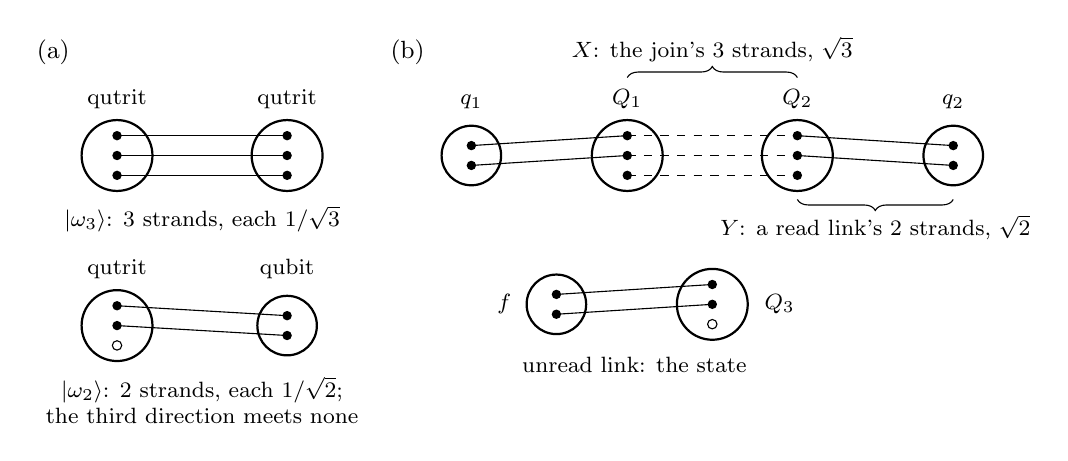
\begin{tikzpicture}[scale=0.9, every node/.style={font=\footnotesize}, dot/.style={circle, fill=black, inner sep=0pt, minimum size=3.4pt}, odot/.style={circle, draw, fill=white, inner sep=0pt, minimum size=3.4pt}]
\draw[thick] (0,0) circle (0.5);
\draw[thick] (2.4,0) circle (0.5);
\foreach \y in {0.28,0,-0.28} {\draw (0,\y) -- (2.4,\y); \node[dot] at (0,\y) {}; \node[dot] at (2.4,\y) {};}
\node at (0,0.8) {qutrit};
\node at (2.4,0.8) {qutrit};
\node at (1.2,-0.9) {$\ket{\omega_{3}}$: $3$ strands, each $1/\sqrt{3}$};
\draw[thick] (0,-2.4) circle (0.5);
\draw[thick] (2.4,-2.4) circle (0.42);
\draw (0,-2.12) -- (2.4,-2.26);
\draw (0,-2.4) -- (2.4,-2.54);
\node[dot] at (0,-2.12) {}; \node[dot] at (0,-2.4) {}; \node[odot] at (0,-2.68) {};
\node[dot] at (2.4,-2.26) {}; \node[dot] at (2.4,-2.54) {};
\node at (0,-1.6) {qutrit};
\node at (2.4,-1.6) {qubit};
\node[align=center] at (1.2,-3.45) {$\ket{\omega_{2}}$: $2$ strands, each $1/\sqrt{2}$;\\the third direction meets none};
\node[font=\small] at (-0.9,1.45) {(a)};
\draw[thick] (5,0) circle (0.42);
\draw[thick] (7.2,0) circle (0.5);
\draw[thick] (9.6,0) circle (0.5);
\draw[thick] (11.8,0) circle (0.42);
\draw (5,0.14) -- (7.2,0.28);
\draw (5,-0.14) -- (7.2,0);
\foreach \y in {0.28,0,-0.28} {\draw[dashed] (7.2,\y) -- (9.6,\y);}
\draw (9.6,0.28) -- (11.8,0.14);
\draw (9.6,0) -- (11.8,-0.14);
\foreach \y in {0.28,0,-0.28} {\node[dot] at (7.2,\y) {}; \node[dot] at (9.6,\y) {};}
\foreach \y in {0.14,-0.14} {\node[dot] at (5,\y) {}; \node[dot] at (11.8,\y) {};}
\node at (5,0.75) {$q_{1}$};
\node at (7.2,0.8) {$Q_{1}$};
\node at (9.6,0.8) {$Q_{2}$};
\node at (11.8,0.75) {$q_{2}$};
\draw[decorate, decoration={brace, amplitude=4pt}] (7.2,1.1) -- (9.6,1.1);
\node at (8.4,1.5) {$X$: the join's $3$ strands, $\sqrt{3}$};
\draw[decorate, decoration={brace, amplitude=4pt, mirror}] (9.6,-0.62) -- (11.8,-0.62);
\node at (10.7,-1.02) {$Y$: a read link's $2$ strands, $\sqrt{2}$};
\draw[thick] (8.4,-2.1) circle (0.5);
\draw[thick] (6.2,-2.1) circle (0.42);
\draw (8.4,-1.82) -- (6.2,-1.96);
\draw (8.4,-2.1) -- (6.2,-2.24);
\node[dot] at (8.4,-1.82) {}; \node[dot] at (8.4,-2.1) {}; \node[odot] at (8.4,-2.38) {};
\node[dot] at (6.2,-1.96) {}; \node[dot] at (6.2,-2.24) {};
\node[anchor=west] at (9.0,-2.1) {$Q_{3}$};
\node[anchor=east] at (5.7,-2.1) {$f$};
\node at (7.3,-2.95) {unread link: the state};
\node[font=\small] at (4.1,1.45) {(b)};
\end{tikzpicture}
\caption{The computation in strands. (a)~A pair of dimension $d$ as $d$ strands, one for each term of $\ket{\omega_{d}}$, Eq.~(\ref{eq:pair}) of the Letter, each of amplitude $1/\sqrt{d}$. A qutrit and a qubit share two strands; the qutrit's third direction (hollow) meets none. (b)~The object of Fig.~\ref{fig:link}(a) in strands, with the shared qutrit drawn as its three copies $Q_{1}$, $Q_{2}$, $Q_{3}$, one per link: the read links $q_{1}Q_{1}$ and $Q_{2}q_{2}$, two strands each; the join of $Q_{1}$ with $Q_{2}$, the qutrit pair $\ket{\omega_{3}}$, three strands (dashed); and the unread link $Q_{3}f$, which carries the state. A path from $q_{1}$ to $q_{2}$ crosses three strands, with amplitude $1/(2\sqrt{3})$, and its two paths give $\ket{\omega_{2}}_{q_{1}q_{2}}/\sqrt{6}$. Both exchanges act on the slots as the mirror of the drawing, the exchange of reads $X$ on records with both letters on ends of one kind and the exchange of links $Y$ on those with one letter at a copy and one at a qubit. A record that survives $X$ runs over the join's three strands and carries $\sqrt{3}$, the qubit--qubit records included, by the clause of Table~\ref{tab:inputs} that a read is an act at the end at which it is taken; one that survives $Y$ runs over a read link's two and carries $\sqrt{2}$. The strands are drawn in a basis; the amplitudes, counts, and weights do not depend on it.}
\label{fig:s-strands}
\end{figure}


\emph{A pair.} A pair of dimension $d$ is $d$ strands, one for each term of Eq.~(\ref{eq:pair}) of the Letter, each joining direction $i$ at one end to direction $i$ at the other with amplitude $1/\sqrt{d}$. A qutrit and a qubit share two strands, and the qutrit's third direction meets none [Fig.~\ref{fig:s-strands}(a)]. Following a strand through several pairs multiplies their amplitudes, and summing over the strands that join the same two ends contracts the shared indices; that is Eq.~(\ref{eq:s-swap}).

\emph{The joint state.} In the object the shared qutrit is drawn as its three copies [Fig.~\ref{fig:s-strands}(b)]. A path from $q_{1}$ to $q_{2}$ crosses a strand of the first read link, one of the join $\ket{\omega_{3}}$ and one of the second read link, with amplitude $\tfrac{1}{\sqrt{2}}\cdot\tfrac{1}{\sqrt{3}}\cdot\tfrac{1}{\sqrt{2}}=\tfrac{1}{2\sqrt{3}}$, and the two paths give $\ket{\omega_{2}}_{q_{1}q_{2}}/\sqrt{6}$, whose norm the factor $\sqrt{6}$ of the joint state restores. The normalized state has $3\cdot 2\cdot 2=12$ terms, each of amplitude $1/(2\sqrt{3})$.

\emph{The counts.} A letter is a box on the strands at one of the four slots, one of $8$ at a copy and one of $3$ at a qubit, and a product record is two boxes at distinct slots, $169$ in all. Swapping the two reads' slots is the mirror of the drawing, and both exchanges act on the slots this way, $X$ on the placements with both boxes on ends of one kind and $Y$ on those with one box at a copy and one at a qubit. A placement and its mirror image coincide or pair up, so $n$ placements with $f$ self-images give $(n+f)/2$ even and $(n-f)/2$ odd combinations: $(169-11)/2=79$ odd, $(73+11)/2=42$ even with both boxes on ends of one kind, and $96/2=48$ even with one box at a copy and one at a qubit, the sizes of Lemma~\ref{lem:s-sectors}. The commutator records concern the reads, not the boxes: two reads in different bases commute up to the sign $-1$ at a qubit, which gives the three commutator records there, and only up to a cube root of unity at the qutrit, which gives none at the copies (Corollary~\ref{cor:s-known}, Theorem~\ref{thm:s-further}).

\emph{The weights.} A record that survives an exchange runs over all the strands of the pair at the end where that exchange acts, $d$ strands of amplitude $1/\sqrt{d}$, so it carries $d\cdot(1/\sqrt{d})=\sqrt{d}$, as in Theorem~\ref{thm:s-gain}(i): over the join's three strands for $X$, $\sqrt{3}$, and over a read link's two for $Y$, $\sqrt{2}$; the three commutator records survive both and carry $\sqrt{6}$.

\emph{The denominator.} A decoration of the object puts a basis operator, the identity included, at each end of a read link, $9\cdot 4=36$ choices at each read link, and a traceless basis operator at each end of the unread link, $8\cdot 3=24$ choices, so the decorations are a basis of $R$, $N=24\cdot 36\cdot 36$ of them (Lemma~\ref{lem:s-register}). The bare insertion weighs each decoration once; the dressed insertion weighs the $172$ records, each by the strands it runs over.

The picture makes the clauses of Table~\ref{tab:inputs} visible but does not supply them: that $X$ runs over the join even at the qubit--qubit records is the clause that a read is an act at the end at which it is taken, and that the denominator counts every decoration is the unit of Lemma~\ref{lem:s-unit}. The strands are drawn in a basis, which $U\otimes\bar{U}$ at the two ends of a pair leaves free; the amplitudes, counts, and weights do not depend on it.

\section{The on-shell correspondence}
\label{sec:s-onshell}

Read off the model, the two-point function of the link factorizes as in field theory,
\begin{equation}
\frac{G_{\mathrm{dressed}}}{G_{\mathrm{bare}}}=Z_{3}\Big(\frac{Z_{2}}{Z_{1}}\Big)^{2}\alpha_{\mathrm{bare}},
\end{equation}
with each factor an output of the same computation. $\alpha_{\mathrm{bare}}=1$: the bare link transmits with certainty, the unit insertion at its two reads on the pair ket giving $\tfrac{1}{2}+\tfrac{1}{2}=1$. This unit and the identity of $R$, which normalizes the trace in $Z_{3}$, are different objects; both read one by the choice of unit, not by being the same insertion. $Z_{2}/Z_{1}=1$ by Lemma~\ref{lem:s-conserved}, and $Z_{3}=\tr_{R}M/N$ is the normalized readout of Eq.~(\ref{eq:readout}).

In the on-shell scheme the coupling is defined by two conditions: the residue of the propagator at the physical pole is one, and the vertex is taken at the pole. The model meets the first through its unit. It supplies the residue that the on-shell scheme normalizes, set to one by the unit of the readout, under whose trace form (Lemma~\ref{lem:s-unit}) the identity reads one, and it constructs no propagator. The second condition, the vertex at the pole at zero transfer, enters with the Photon Conjecture of the Letter, and the model constructs no function of the momentum transfer. The model's counterpart of decoupling, the statement that charged states beyond the scale of measurement leave the zero-transfer limit unchanged, is that the readout dimension of the link is a function of its own two ends, so no readout dimension beyond the link enters. Table~\ref{tab:s-onshell} sets out the correspondence row by row, and Fig.~\ref{fig:s-roles} draws its first two rows. The two definitions of the computed quantity, the two-point configuration and the normalized readout with its units, are the model's counterparts of its first three rows.

\begin{table}[h]
\caption{The on-shell scheme and its counterparts in the model.}
\label{tab:s-onshell}
\footnotesize
\begin{ruledtabular}
\begin{tabular}{>{\raggedright\arraybackslash}p{0.44\linewidth}>{\raggedright\arraybackslash}p{0.50\linewidth}}
on-shell QED & the model \\ \hline
photon two-point function: two field insertions on the vacuum & two reads of the link on a third, unread link that carries the state (Sec.~\ref{sec:s-config}(b)) \\
$\alpha(0)=Z_{3}\,\alpha_{\mathrm{bare}}$: dressed over bare, at the pole & $\tr_{R}M/\tr_{R}\openone_{R}$: dressed over bare insertion (Theorem~\ref{thm:s-readout}) \\
coupling per unit charge; $Z_{1}=Z_{2}$ by the Ward identity & units at one scale, $\mathcal{Q}$ reading one at a ket end (Lemma~\ref{lem:s-unit}); $Z_{2}/Z_{1}=1$ by conservation (Lemma~\ref{lem:s-conserved}) \\
zero momentum transfer; a massless pole & enter with the Photon Conjecture; the model constructs no propagator \\
\end{tabular}
\end{ruledtabular}
\end{table}

\begin{figure}[h]
\centering
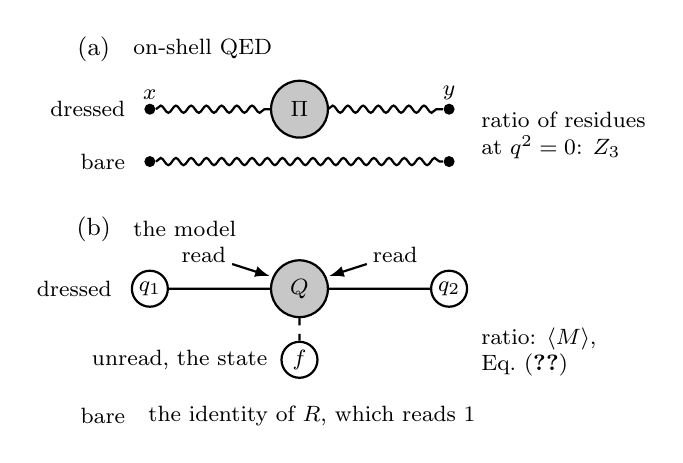
\begin{tikzpicture}[scale=0.95, every node/.style={font=\footnotesize},
  photon/.style={decorate, decoration={snake, amplitude=1.3pt, segment length=5.5pt}, thick},
  ins/.style={circle, fill=black, inner sep=0pt, minimum size=4pt},
  qd/.style={circle, draw, thick, fill=white, inner sep=0pt, minimum size=13pt}]
% (a) on-shell QED
\node[font=\small] at (-0.75,1.15) {(a)};
\node[anchor=west] at (-0.35,1.15) {on-shell QED};
\node[anchor=east] at (-0.2,0.35) {dressed};
\node[ins] (x) at (0,0.35) {}; \node[ins] (y) at (4,0.35) {};
\draw[photon] (x) -- (1.62,0.35);
\draw[photon] (2.38,0.35) -- (y);
\draw[thick, fill=black!22] (2,0.35) circle (0.38);
\node at (2,0.35) {$\Pi$};
\node[above] at (x) {$x$}; \node[above] at (y) {$y$};
\node[anchor=east] at (-0.2,-0.35) {bare};
\node[ins] (xb) at (0,-0.35) {}; \node[ins] (yb) at (4,-0.35) {};
\draw[photon] (xb) -- (yb);
\node[anchor=west, align=left] at (4.3,0) {ratio of residues\\at $q^{2}=0$: $Z_{3}$};
% (b) the model
\node[font=\small] at (-0.75,-1.25) {(b)};
\node[anchor=west] at (-0.35,-1.25) {the model};
\node[anchor=east] at (-0.38,-2.05) {dressed};
\node[qd] (q1) at (0,-2.05) {$q_{1}$};
\node[qd] (q2) at (4,-2.05) {$q_{2}$};
\draw[thick, fill=black!22] (2,-2.05) circle (0.38);
\node at (2,-2.05) {$Q$};
\draw[thick] (q1) -- (1.62,-2.05);
\draw[thick] (2.38,-2.05) -- (q2);
\draw[-latex, thick] (1.1,-1.72) -- (1.6,-1.88); \node at (0.72,-1.6) {read};
\draw[-latex, thick] (2.9,-1.72) -- (2.4,-1.88); \node at (3.28,-1.6) {read};
\node[qd] (f) at (2,-3.0) {$f$};
\draw[thick, dashed] (2,-2.43) -- (f);
\node[anchor=east] at (1.7,-3.0) {unread, the state};
\node[anchor=west, align=left] at (4.3,-2.9) {ratio: $\langle M\rangle$,\\Eq.~(\ref{eq:alpha})};
\node[anchor=east] at (-0.2,-3.75) {bare};
\node[anchor=west] at (-0.15,-3.75) {the identity of $R$, which reads $1$};
\end{tikzpicture}
\caption{A correspondence of roles, not of diagrams. (a)~In on-shell QED, $Z_{3}$ is the residue at $q^{2}=0$ of the dressed photon two-point function, two field insertions at $x$ and $y$ joined through every vacuum-polarization insertion (shaded), over that of the bare one. (b)~The model's counterpart in the object of Fig.~\ref{fig:link}(a), with the two read links drawn apart: the two reads, taken at the shared qutrit $Q$ on the links to $q_{1}$ and $q_{2}$, are the two insertions, the unread link to $f$ carries the state, the bare insertion is the identity of $R$, and the dressed insertion $M$ weighs the $172$ records at $Q$ (shaded), Eq.~(\ref{eq:alpha}) of the Letter. No record is a Feynman diagram. The model has no charged loop, no vertex factor, no loop momentum, and no expansion in a coupling, and the identification of the object with the photon is the Photon Conjecture.}
\label{fig:s-roles}
\end{figure}


\textbf{The one definitional identification.} That the dressed readout of the two reads is a two-point function in the sense of field theory, read in the on-shell scheme, is a definition. It names what Theorem~\ref{thm:value} of the Letter computes and is used in no proof. It is distinct from the model's own definition of a two-point function, Sec.~\ref{sec:s-config}(b), which selects the configuration that is read and so enters the computation. The names \emph{vacuum polarization}, \emph{zero momentum transfer}, and \emph{Thomson limit} are those of the field-theory quantities that the correspondence and the conjecture point to; the structures they presuppose in field theory, a field over spacetime and a scattering amplitude, are not supplied here.

\section{What else the count could have given}
\label{sec:s-alternatives}

Table~\ref{tab:s-alternatives} lists the alternatives that would change the number, with the reason each is excluded. No exclusion refers to the measured value of $\alpha$. The configurations other than the object are excluded by the end rule, the definition of the two-point function, or the absence of an acting charge (Sec.~\ref{sec:s-config}), so the table gives a value for a configuration only where one is in hand.

\begin{table}[h]
\caption{Alternatives that change the number, the value each gives, and why each is excluded. The computed value is the first row. Inverses are of the readout.}
\label{tab:s-alternatives}
\footnotesize
\begin{ruledtabular}
\begin{tabular}{>{\raggedright\arraybackslash}p{0.30\linewidth}>{\raggedright\arraybackslash}p{0.21\linewidth}>{\raggedright\arraybackslash}p{0.09\linewidth}>{\raggedright\arraybackslash}p{0.32\linewidth}}
alternative & value & inverse & excluded by \\ \hline
computed: $X$ at the qutrit end, $Y$ at the qubit end, weights $\sqrt{k_{r}}$ & $\frac{79+48\sqrt{2}+42\sqrt{3}+3\sqrt{6}}{31104}$ & $137.036$ & --- \\
the two ends swapped & $\frac{79+42\sqrt{2}+48\sqrt{3}+3\sqrt{6}}{31104}$ & $135.894$ & the end rule, a clause of the definition of a read (Theorem~\ref{thm:s-gain}(ii)) \\
both exchanges at the qubit end & $\frac{85+90\sqrt{2}}{31104}$ & $146.524$ & the end rule (Theorem~\ref{thm:s-gain}(ii)) \\
both exchanges at the qutrit end & $\frac{88+90\sqrt{3}}{31104}$ & $127.536$ & the copies of the shared qutrit are one qudit, so the exchange of links moves only the qubits (Theorem~\ref{thm:s-gain}(ii)) \\
the exchange of reads placed where the letters sit & $\frac{85+54\sqrt{2}+36\sqrt{3}}{31104}$ & $139.030$ & a read is an act at the end at which it is taken (Theorem~\ref{thm:s-gain}(ii)) \\
qubit--qubit records counted as moved by the exchange of links & $\frac{79+48\sqrt{2}+36\sqrt{3}+9\sqrt{6}}{31104}$ & $134.485$ & they occupy the same two qubits after it (Theorem~\ref{thm:s-gain}(ii)) \\
the copies of the shared qutrit as separate qudits & $\frac{79+42\sqrt{3}+51\sqrt{6}}{31104}$ & $112.423$ & a shared qudit is one qudit (Theorem~\ref{thm:s-gain}(ii)) \\
survival without the record's own sign & $\frac{82+48\sqrt{2}+42\sqrt{3}}{31104}$ & $139.713$ & the definition of the known gives commutator records the order sign (Theorem~\ref{thm:s-further}) \\
commutator records survive $X$ only & $\frac{79+48\sqrt{2}+45\sqrt{3}}{31104}$ & $138.348$ & the exchange of links moves them between the read qubits (Theorem~\ref{thm:s-further}) \\
sums and differences of the commutators both kept & $\frac{79+48\sqrt{2}+42\sqrt{3}+6\sqrt{6}}{31104}$ & $132.739$ & the sums read $+1$, not the order sign (Theorem~\ref{thm:s-further}) \\
no commutator records & $\frac{79+48\sqrt{2}+42\sqrt{3}}{31104}$ & $141.621$ & the definition of the known (Corollary~\ref{cor:s-known}) \\
Born weights $k_{r}$ instead of $\sqrt{k_{r}}$ & $\frac{319}{31104}$ & $97.505$ & four letters, a four-point quantity, not the two-point function (Theorem~\ref{thm:s-gain}(i)) \\
count of read ends instead of units of charge & $\frac{158+96\sqrt{2}+82\sqrt{3}+3\sqrt{6}}{31104}$ & $70.190$ & not a coupling per unit of the conserved count (Theorem~\ref{thm:s-ward}) \\
normalized by the $172$ records instead of $N$ & $\frac{79+48\sqrt{2}+42\sqrt{3}+3\sqrt{6}}{172}$ & $0.758$ & a coupling per record, not per unit of the conserved count (Lemma~\ref{lem:s-unit}) \\
no weights & $\frac{172}{31104}$ & $180.837$ & the factor $\sqrt{d}$ where a record survives an exchange (Theorem~\ref{thm:s-gain}(i)) \\
smallest readable configuration: two $(2,2)$ reads at a shared qubit & $\frac{30+30\sqrt{2}}{256}$ & $3.535$ & $(2,2)$ carries no acting charge (Lemma~\ref{lem:s-center}); no unread link (b) \\
two $(2,3)$ reads at a shared qubit with a $(2,3)$ unread link (same readout dimension, $174$ records) & not evaluated & --- & reads at the qubit end of a $(2,3)$ link, the end rule (a) \\
the other configurations of Table~\ref{tab:s-configs} & not evaluated & --- & the end rule (a), the two-point definition (b), or no acting charge (Sec.~\ref{sec:s-config}) \\
\end{tabular}
\end{ruledtabular}
\end{table}

Two alternatives land within one percent of the computed value: the ends swapped, which the end rule excludes, and the commutator records at $X$ alone, which the exchange of links excludes, since it moves them between the read qubits.

\section{The explicit matrices}
\label{sec:s-matrices}

\textbf{The pair ket.} On the six-dimensional tensor space of the link, indexed by the qubit direction times three plus the qutrit direction, the flat ket is $\sqrt{2}\ket{\omega_{2}}=(1,0,0,0,1,0)$, with squared norm $2$. Its Gram matrix has trace $2$, squares to twice itself, and has rank one.

\textbf{The identification algebra.} On $\mathbb{C}^{2}\oplus\mathbb{C}^{3}$, with indices $0,1$ at the qubit block and $2,3,4$ at the qutrit block, and $E_{ab}$ the matrix units, the basis is
$e_{1}=E_{01}-E_{10}$, $e_{2}=i(E_{01}+E_{10})$, $e_{3}=i(E_{00}-E_{11})$;
$e_{4}=E_{23}-E_{32}$, $e_{5}=E_{24}-E_{42}$, $e_{6}=E_{34}-E_{43}$, $e_{7}=i(E_{23}+E_{32})$, $e_{8}=i(E_{24}+E_{42})$, $e_{9}=i(E_{34}+E_{43})$, $e_{10}=i(E_{22}-E_{33})$, $e_{11}=i(E_{33}-E_{44})$;
and $e_{12}=\mathcal{Q}=i\,\mathrm{diag}(3,3;\,-2,-2,-2)$. The first three span $su(2)$, the next eight $su(3)$, and the last $u(1)$. The action of the twelve on the pair ket, as a $12\times 12$ integer matrix of the real and imaginary parts of the six entries, has rank $8$.

\textbf{The stabilizer and its center.} The null space of that action has the basis
\begin{equation}
e_{1}+e_{4},\qquad e_{2}-e_{7},\qquad e_{3}-e_{10},\qquad e_{3}+2e_{11}-e_{12}.
\end{equation}
The center of this subalgebra is the line of $-8e_{10}-16e_{11}+8e_{12}$, whose diagonal is $24\,(1,1,-1,-1,0)$, a multiple of $\mathcal{U}$.

\textbf{The joint state.} With the copies $Q_{1},Q_{2},Q_{3}$ of the shared qutrit,
\begin{equation}
\ket{\omega_{2}}_{Q_{1}q_{1}}\ket{\omega_{2}}_{Q_{2}q_{2}}=\tfrac{1}{2}\sum_{i,j=1}^{2}\ket{i}_{Q_{1}}\ket{i}_{q_{1}}\ket{j}_{Q_{2}}\ket{j}_{q_{2}},\qquad (P_{3})_{Q_{1}Q_{2}}\ket{ij}=\frac{\delta_{ij}}{\sqrt{3}}\ket{\omega_{3}},
\end{equation}
so the projected vector is $\frac{1}{2\sqrt{3}}\ket{\omega_{3}}_{Q_{1}Q_{2}}(\ket{11}+\ket{22})_{q_{1}q_{2}}$, of squared norm $1/6$. Multiplying by the unread link and by $\sqrt{6}$ gives $\ket{\Omega}$: $3\cdot 2\cdot 2=12$ terms of amplitude $1/(2\sqrt{3})$, with $12\cdot\frac{1}{12}=1$.

\textbf{The matchings.} $G_{2}$ is generated by the transposition and the phases $\mathrm{diag}(i,1)$ and $\mathrm{diag}(1,i)$, and has order $32$. $G_{3}$ is generated by the two adjacent transpositions and the three phases $\mathrm{diag}(i,1,1)$, $\mathrm{diag}(1,i,1)$, and $\mathrm{diag}(1,1,i)$, and has order $384$. $\mathcal{Q}$ commutes with each of the $4+9=13$ matrix units of the block algebra and is fixed by every matching.

\section{Formalization}
\label{sec:s-lean}
\begin{table}[!htbp]
\caption{Results of this paper and their declarations in \texttt{ChainAlpha.lean}. Axioms are as reported by \texttt{\#print axioms}, combined over the declarations of each row: P propositional extensionality, Q quotient soundness, C choice; --- none.}
\label{tab:s-lean}
\footnotesize
\begin{ruledtabular}
\begin{tabular}{>{\raggedright\arraybackslash}p{0.38\linewidth}>{\raggedright\arraybackslash}p{0.47\linewidth}>{\raggedright\arraybackslash}p{0.08\linewidth}}
result & declaration & axioms \\ \hline
the value, Eq.~(\ref{eq:alpha}) of the Letter; the object as a two-point configuration & \lean{main}, \lean{dressing_of_the_qutrit_qubit_link} & P \\
readout dimension $24\cdot 36\cdot 36$, the readout-dimension rule evaluated & \lean{readout_dimension} & --- \\
$169$ products and $172$ records (Corollary~\ref{cor:s-records}) & \lean{product_count}, \lean{record_count} & P \\
the records orthogonal, hence independent & \lean{records_orthogonal} & P, Q \\
sector sizes, and the polynomials at $a=8$, $b=3$ (Lemma~\ref{lem:s-sectors}) & \lean{sectors}, \lean{sector_polynomials} & P \\
weight factors $3$ and $2$; the exchange of links leaves the shared qutrit in place and swaps the qubits (Theorem~\ref{thm:s-gain}) & \lean{weight_factors} & P \\
the two exchanges agree with Eq.~(\ref{eq:s-exchanges}) at all $172$ records & \lean{exchanges_agree_with_pairings}, \lean{exchange_domains} & P \\
end rule & \lean{end_rule}, \lean{fixesFar_iff_le} & P \\
anticommutation at a qubit and the three commutator records (Corollary~\ref{cor:s-known}, Theorem~\ref{thm:s-further}) & \lean{weyl_sign}, \lean{commutators_single}, \lean{commutator_records} & P \\
every record an eigenvector of the exchange (Corollary~\ref{cor:s-records}) & \lean{records_exchange_eigenbasis} & P \\
$\mathcal{Q}$ acts as $i\openone$ on the link and spans the center; $\mathcal{Q}=6iY$ (Lemma~\ref{lem:s-center}) & \lean{Q_on_link}, \lean{Q_central}, \lean{center_one_dimensional}, \lean{Q_is_six_i_Y} & P \\
stabilizer: rank $8$, dimension $4$, center the line of $\mathcal{U}$ (Theorem~\ref{thm:s-stabilizer}) & \lean{action_rank}, \lean{stab_independent}, \lean{stab_center_one_dimensional} & P \\
unit of the count, $B(\mathcal{Q},\mathcal{Q})=1$ (Lemma~\ref{lem:s-unit}) & \lean{unit_of_the_count} & P \\
selection of the link under the cited read cap of the Letter & \lean{selection_under_read_cap} & P, Q, C \\
the readers reproduce the cap; conjugation at a qubit and at a qutrit (Sec.~\ref{sec:s-read}) & \lean{readers_reproduce_the_cap}, \lean{qubit_absorbs_conjugation}, \lean{qutrit_conjugation_obstruction} & P, Q, C \\
uniqueness of the configuration, Theorem~\ref{thm:object} of the Letter, and the object's configuration (Sec.~\ref{sec:s-config}) & \lean{configuration_unique}, \lean{object_config_of_world} & P, Q, C \\
matching groups of orders $32$ and $384$; commutant of dimension $3$ (Lemmas~\ref{lem:s-matching}, \ref{lem:s-commutant}) & \lean{matching_group_orders}, \lean{commutant_dimension} & P \\
the join's laboratory postselection probability, $1/6$; in the model the join has no failure branch (Sec.~\ref{sec:s-count}) & \lean{join_probability} & --- \\
\end{tabular}
\end{ruledtabular}
\end{table}


The ancillary file \texttt{ChainAlpha.lean} is a single Lean~4 file on the core library alone, with no Mathlib and no imports; \texttt{lean ChainAlpha.lean} checks it with Lean~4.35.0 in about a hundred seconds. Every computation is checked by the kernel. The file contains no \texttt{sorry}, no axiom declaration, and no native code. Its main theorem, \lean{ChainAlpha.main}, has no hypotheses beyond the definitions of the file's Part~1. It states that the object is a two-point configuration of the qutrit--qubit link, that reads at the qutrit fix the qubit while reads at the qubit do not fix the qutrit, that every record, built from the slots and the commutator matrices, is an eigenvector of the exchange of the reads, and that the normalized readout is $(79+48\sqrt{2}+42\sqrt{3}+3\sqrt{6})/31104$. It depends on propositional extensionality alone. The file computes the two traces that define the readout, the sum of $\sqrt{k_{r}}$ over the records and the readout dimension, without constructing the readout space itself.

The definitions of Part~1 are those of Table~\ref{tab:inputs}: the axiom as a structure of qudits and links; its five definitions, with the definition of fix and the three clauses of Table~\ref{tab:inputs}, from which the file builds the slots and their letters, the records with their own signs and the commutator records, the two exchanges and survival, and the weight function; and the two definitions of the computed quantity, the two-point configuration and the normalized readout.
Outside comments, the digits $79$, $48$, $42$, and $31104$ and the counts $169$ and $172$ occur only in theorem statements, so they are outputs and not inputs. Table~\ref{tab:s-lean} maps the results of this paper to the declarations. The ancillary script \texttt{mutations.py} perturbs the definitions one at a time; every perturbation that changes a value at the object makes the main theorem or \lean{commutator_records} fail.

Under the read cap, a named hypothesis that cites the theorems of St{\o}rmer, Woronowicz, and Choi in their numerical form for the definition of a readable type, \lean{selection_under_read_cap} gives the qutrit--qubit link as the only readable type with an acting charge. The file also contains the readers remark of Sec.~\ref{sec:s-read}: \lean{readers_reproduce_the_cap} shows that readability by reads, with the qubit and the qutrit as readers and the far end absorbing the conjugation, holds exactly when $d_{1}d_{2}\leq 6$, so \lean{reads_satisfy_the_read_cap} discharges the cap's hypothesis for it; \lean{qubit_absorbs_conjugation} and \lean{qutrit_conjugation_obstruction} check the two facts about conjugation on the matching groups. The file does not formalize the theorems behind the cap, statements over the full unitary group, the on-shell identification, or the Photon Conjecture, which appears nowhere in it.



\clearpage
\section{Glossary}
\label{sec:s-glossary}

\begin{table}[h]
\caption{Terms of the model and the standard notions they name.}
\label{tab:s-glossary}
\footnotesize
\begin{ruledtabular}
\begin{tabular}{p{0.26\linewidth}p{0.48\linewidth}p{0.18\linewidth}}
term & standard notion & symbol \\ \hline
qudit & finite-dimensional quantum system, of dimension $d\geq 2$ (a one-dimensional system cannot be entangled) & $\mathbb{C}^{d}$ \\
pair, or link, of type $(d_{1},d_{2})$ & two qudits in the maximally entangled state on their common support, admitted by the axiom; the output of distilling them & $\ket{\omega_{m}}$, $m=\min(d_{1},d_{2})$ \\
shared qudit & system at the end of two or more links, carried as one copy per link; its copies are one qudit, so exchanging two links leaves it in place and moves only their far ends & $Q$ \\
distilling & projection onto a maximally entangled pair & $P_{m}$ \\
no failure branch & the projection is the act and has no other outcome; in a laboratory, a postselection & --- \\
read & an act at the end at which it is taken: distillation in a basis of that end, the basis passed to the far end, which it reaches whole, so a read is taken at the larger end & --- \\
fix & determine with certainty on the one copy, leaving nothing open; no expectation value is estimated, and every consistent relation between two fixed ends is of a kind reads carry & --- \\
known & what all reads of a qudit fix jointly, under every matching of its pairs and every exchange of its reads or of its pairs; two anticommuting reads also fix their product, with their order as its sign & --- \\
matching; twirl & local unitary $U\otimes\bar{U}$ fixing the pair; the isotropic twirl & $G_{d}$; $T_{d}$ \\
decomposable map & a completely positive map plus a completely positive map after the transpose & $\Phi_{1}+\Phi_{2}\circ T$ \\
read cap & $d_{1}d_{2}\leq 6$, the readable types: the definition of fix, with the theorems of St{\o}rmer, Woronowicz, and Choi & --- \\
readable type; dark type & a type whose ends admit only decomposable positive maps, $(2,2)$ and $(2,3)$; one whose ends admit a non-decomposable positive map, though its links stay maximally entangled & --- \\
identification algebra & $s(u(d_{1})\oplus u(d_{2}))=su(d_{1})\oplus su(d_{2})\oplus u(1)$; at $(2,3)$ the Lie algebra of $S(U(3)\times U(2))$ & --- \\
acting central charge & center of that algebra, nonzero on the pair; at $(2,3)$ the hypercharge direction & $\mathcal{Q}=6iY$ \\
unbroken generator & center of the stabilizer of the pair & $\mathcal{U}$ \\
configuration; arm & a shared qudit with the links at it, each read or unread & --- \\
end rule & a $(2,3)$ link is read at its qutrit end & --- \\
two-point function & two reads of the link on a third, unread link of its type & --- \\
join & contraction of two links at a shared qudit & --- \\
strand & a term $\ket{i}\ket{i}$ of a pair ket in a chosen basis, of amplitude $1/\sqrt{d}$; an index line of a tensor network & --- \\
decoration & a basis operator at each end of the object, any at a read link and traceless at the unread link; the decorations are a basis of $R$ & --- \\
slot; letter; record & an end of a read link; a basis element of the traceless observables there; product of letters at two slots, or a commutator record & $(8,3,8,3)$; $r$ \\
exchange of reads; of links & exchanging a record's two reads; exchanging the two read links, which leaves the shared qudit in place & $X$; $Y$ \\
own sign; survives; sectors & $+1$ for a product, the order sign for a commutator record; returned times its own sign by an exchange; the joint eigenspaces of $X$ and $Y$ & $\sigma_{r}$ \\
weight & square root of the product of the dimensions of the ends at which the exchanges a record survives act & $\sqrt{k_{r}}$ \\
readout dimension & dimension of the readout algebra of a configuration & $N=\dim R$ \\
readout; bare and dressed insertions & normalized trace over $R$; the identity of $R$; the operator with $\sqrt{k_{r}}$ on each record direction & $\tr_{R}M/N$; $\openone_{R}$; $M$ \\
unit of the readout & trace form on the identification algebra, induced by the readout on $R$ under the left action & $B(\xi,\eta)$ \\
unit of the count & the charge of one ket end, $\mathcal{Q}$ read by left multiplication & $L_{\mathcal{Q}}=i\openone_{R}$ \\
\end{tabular}
\end{ruledtabular}
\end{table}


\end{document}
